\documentclass[final]{fhnwreport}       %[mode] = draft or final
                                        %{class} = fhnwreport, article, 
                                        %          report, book, beamer, standalone
%%---Main Packages-----------------------------------------------------------------------
\usepackage[english, ngerman]{babel}	%Mul­tilin­gual sup­port for LaTeX
\usepackage[T1]{fontenc}				%Stan­dard pack­age for se­lect­ing font en­cod­ings
\usepackage[utf8]{inputenc}				%Ac­cept dif­fer­ent in­put en­cod­ings
\usepackage{lmodern}                    %The newer Font-Set
\usepackage{textcomp}					%LaTeX sup­port for the Text Com­pan­ion fonts
\usepackage{graphicx} 					%En­hanced sup­port for graph­ics
\usepackage{float}						%Im­proved in­ter­face for float­ing ob­jects
\usepackage{ifdraft}                    %Let you check if the doc is in draft mode

%%---Useful Packages---------------------------------------------------------------------
\usepackage[pdftex,dvipsnames,table]{xcolor}  %Driver-in­de­pen­dent color ex­ten­sions for LaTeX
\usepackage{csquotes}                   %Simpler quoting with \enquote{}
\usepackage{siunitx} 					%A com­pre­hen­sive (SI) units pack­age
\usepackage{listings}					%Type­set source code list­ings us­ing LaTeX
\usepackage[bottom]{footmisc}			%A range of foot­note op­tions
\usepackage{footnote}					%Im­prove on LaTeX's foot­note han­dling
\usepackage{verbatim}					%Reim­ple­men­ta­tion of and ex­ten­sions to LaTeX ver­ba­tim
\usepackage[textsize=footnotesize]{todonotes} %Mark­ing things to do in a LaTeX doc­u­ment
\usepackage{booktabs}
\usepackage{lscape}
\usepackage{blindtext}
\usepackage{wrapfig}
\usepackage{caption}
\usepackage{romannum}

%%---Tikz Packages-----------------------------------------------------------------------
\usepackage{standalone}
\usepackage{tikz}
\usepackage{circuitikz}
\usetikzlibrary{arrows}
\usetikzlibrary{calc}
\usetikzlibrary{intersections}

%%---Math Packages-----------------------------------------------------------------------
\usepackage{amsmath}					%AMS math­e­mat­i­cal fa­cil­i­ties for LaTeX
%\usepackage{amssymb}					%Type­set­ting symbols (AMS style)
%\usepackage{array}						%Ex­tend­ing the ar­ray and tab­u­lar en­vi­ron­ments
%\usepackage{amsthm}					%Type­set­ting the­o­rems (AMS style)

%%---Table Packages----------------------------------------------------------------------
\usepackage{tabularx}					%Tab­u­lars with ad­justable-width columns
%\usepackage{longtable}
\usepackage{multirow}					%Create tab­u­lar cells span­ning mul­ti­ple rows
\usepackage{multicol}					%In­ter­mix sin­gle and mul­ti­ple columns

%%---PDF / Figure Packages---------------------------------------------------------------
\usepackage{pdfpages}					%In­clude PDF doc­u­ments in LaTeX
\usepackage{pdflscape}					%Make land­scape pages dis­play as land­scape
\usepackage{subfig}					    %Fig­ures di­vided into sub­fig­ures

%%---Other Packages----------------------------------------------------------------------
%\usepackage{xargs}                     %De­fine com­mands with many op­tional ar­gu­ments

%%---Bibliography------------------------------------------------------------------------
\usepackage[style=ieee,urldate=comp,backend=biber]{biblatex}
\addbibresource{literature/bibliography.bib}

%%---Main Settings-----------------------------------------------------------------------
\graphicspath{{./graphics/}}			%Defines the graphicspath
%\geometry{twoside=false}				    %twoside=false disables the "bookstyle"
\setlength{\marginparwidth}{2cm}
\overfullrule=5em						%Creates a black rule if text goes over the margins => debugging


%%---User Definitions--------------------------------------------------------------------
%%Tabel-Definitions: (requires \usepackage{tabularx})
\newcolumntype{L}[1]{>{\raggedright\arraybackslash}p{#1}}    %column-width and alignment
\newcolumntype{C}[1]{>{\centering\arraybackslash}p{#1}}
\newcolumntype{R}[1]{>{\raggedleft\arraybackslash}p{#1}}

%%---Optional Package Settings-----------------------------------------------------------
%Listings-Settings: (requires \usepackage{listings}) => Example with Matlab Code
\lstset{language=Matlab,%
    basicstyle=\footnotesize\ttfamily,
    breaklines=false,%
    morekeywords={switch, case, otherwise},
    keywordstyle=\color{Blue},%
    tabsize=2,
    %morekeywords=[2]{1}, keywordstyle=[2]{\color{black}},
    identifierstyle=\color{Black},%
    stringstyle=\color{Purple},
    commentstyle=\color{Green},%
    showstringspaces=false,%without this there will be a symbol in the places where there is a space
    numbers=left,%
    numberstyle={\tiny \color{black}},% size of the numbers
    numbersep=9pt, % this defines how far the numbers are from the text
    %emph=[1]{word1, word2,...},emphstyle=[1]\color{red}
}										                %loads all packages, definitions and settings												
\title{\Huge{\textbf{Fachbericht}}\\}          %Project Title
\author{\huge{Wetterstation mit Solar Energie}}          %Document Type => Technical Report, ...
\date{Windisch, \today}             %Place and Date


\begin{document}

%%---TITLEPAGE---------------------------------------------------------------------------
\selectlanguage{ngerman}                %ngerman or english
\maketitle
%\vspace*{-1cm}
\vspace*{-0.5cm}						    %compensates the space after the date line.
\vfill
\begin{figure}[H]
\centering
%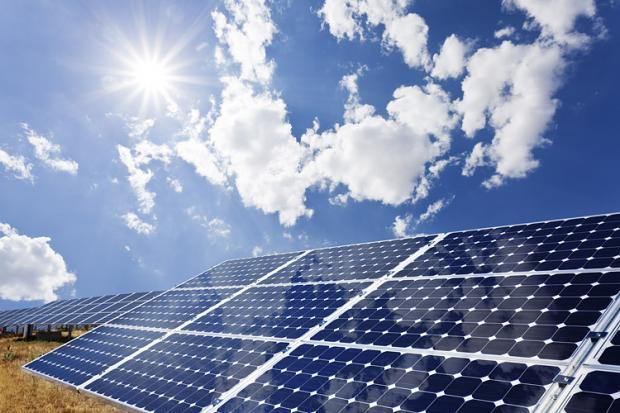
\includegraphics[width=\linewidth]{Titelbild.jpg}
\end{figure}
\vfill

{
\renewcommand\arraystretch{2}
\begin{center}
\begin{tabular}{>{\bf}p{4cm} l}
Hochschule                 &    Hochschule für Technik - FHNW\\
Studiengang                &    Elektro- und Informationstechnik\\
Autor/-en  		           & 	Mischa Knupfer, Andres Minder\\
Betreuer                   &    Prof. Dr. Taoufik Nouri\\
Auftraggeber               &    Prof. Dr. Taoufik Nouri\\
Version                    &    1.2 %Normally not used!
\end{tabular}
\end{center}
}

\clearpage
			
%%---ABSTRACT----------------------------------------------------------------------------
\selectlanguage{english}				%ngerman or english
\thispagestyle{empty}
\begin{abstract}
\noindent
Climate and weather data are the main sources to determine plots for specific plants or plant species for a specific climate. Because of that, farmers need to know the climate and weather data to optimize their work. Swiss farmers have the advantage of getting this information through a federal agency, which does not apply to farmers in subtropical areas. To provide these information for farmers in subtropical areas, a low-priced mobile weather station is required. This project should design a prototype of a weather station, which can record data for air temperature, Rainfall, wind strength and hours of sunshine. In addition to that, the DS3231 real time clock (RTC) should generate a timestamp to the data before it is stored in the data memory. The core of the weather station is the microcontroller ArduinoMega2560, which contains the program code and manages the data storage. The wind strength is being measured by the WD123 from Froggit, the rainfall by an ombrometer from Misol and the air temperature by the BME280 from Bosch that measures also humidity and pressure of the air. Moreover, a wind vane (p/n 80422) from Argent Data Systems allows the weather station to determine the wind direction. Those gained data points are stored on an internal microSD card.\\[0.5cm]
The mobile weather station is able to provide data for temperature, humidity and pressure of the air as well as the Rainfall and the strength and direction of the wind. Furthermore, the mobile weather station is also able to store the data points with timestamp on the microSD card. In a further project, a battery will be implemented which will be supported by photovoltaic. Furthermore, GPS and data query over SMS (GSM) will also be implemented in that further project.\\
\\
Key Words: mobile weather station, sensors, microSD card, GPS, SMS (GSM)


\end{abstract}	

%%---TABLE OF CONTENTS-------------------------------------------------------------------
\pagenumbering{Roman}		
\selectlanguage{ngerman}				%ngerman or english
\tableofcontents
\clearpage

%%---TEXT--------------------------------------------------------------------------------
\pagenumbering{arabic}
\section{Einleitung}
Pflanzen benötigen eine ihnen entsprechende Umwelt. Durch meteorologische Messdaten kann diese ermittelt und durch Agronome optimal bewirtschaftet werden. Ausserdem können bei genügend Messdaten aus einem Erfassungsnetz Wetterprognosen erstellt werden. Die Erhebung solcher Messdaten trägt somit erheblich zum wirtschaftlichen Erfolg in der Agronomie bei und kann bei einem geeignet grossen Erfassungsnetz Bewohner vor Unwetter warnen. In den ärmeren Teilen Afrikas und Südamerikas sind solche Systeme jedoch nicht verbreitet.\\[0.5cm]
Aus diesem Grund soll eine kostengünstige, erweiterbare und mobile Wetterstation gebaut werden, welche die örtlichen Agronomen unterstützt. Diese Wetterstation soll die Niederschlagsmenge, die Windstärke, die Lufttemperatur und die Sonnenstunden messen können. Ausserdem soll die Wetterstation mittels Photovoltaik unterstützt werden, und erhobene Daten via SMS abrufbar sein. Mit einem GPS-Modul soll der Standort der mobilen Wetterstation erfasst werden. Im Projekt 5 wird ein erster Prototyp erstellt, welcher die Datenermittlung mit der Sensorik und Datenspeicherung beinhaltet. Die Stromversorgung (Akku, Solarpanels), das GPS und das Senden der Daten über SMS werden im Projekt 6 implementiert.\\[0.5cm]
Die Lufttemperatur wird über den Temperatursensor XYZ gemessen. Mittels Kipplöffelprinzip wird die Niederschlagsmenge über den Sensor XYZ ermittelt, wobei die Funktionsweise des Kipplöffels zuerst mit einem Selbstbau überprüft wird. Die Windstärke wird über das Anemometer XYZ eruiert. Um die Sonnenstunden zu ermitteln werden zwei Varianten (zum einen via Ladestrom der Photovoltaikanlage, zum anderen mit einem Sensor XYZ) verglichen und die Leistungsärmere implementiert, was jedoch erst im Projekt 6 stattfindet. Es wird für das Prototyping ein ArduinoMega2560 verwendet, welcher die Sensoren über die vorhandenen Peripherieanschlüsse mit dem Mikrocontroller verbindet. Die gesammelten Daten werden auf einer microSD Karte abgespeichert, wobei mit Hilfe eines RTC (Real Time Clock) ein Zeitstempel hinzugefügt wird.\\[0.5cm]
Das Projekt 5 liefert die erwünschten Messdaten von Lufttemperatur, Windgeschwindigkeit und Niederschlagsmenge. Zusätzlich werden Luftdruck, Luftfeuchtigkeit und Windrichtung gemessen. Ausserdem werden die Daten wunschgemäss auf einer microSD Karte, mit zugehörigem Zeitstempel versehen, gespeichert.\\[0.5cm]
Der nachfolgende Bericht beinhaltet die Auftragsbeschreibung (Kapitel \ref{chap:Auftrag}) und die festgelegten Ziele (Kapitel \ref{chap:Ziele}), sowie die Kapitel MCU (Kapitel \ref{chap:MCU}), RTC (Kapitel \ref{chap:RTC}), Sensoren (Kapitel \ref{chap:Sensoren}) und Datenspreicherung (Kapitel \ref{chap:data}), in welchen die einzelnen Elemente der mobilen Wetterstation thematisiert werden. Zuletzt folgt das Kapitel Konzeptvalidierung (Kapitel \ref{chap:valid}), worin die Funktionalität des Konzepts der mobilen Wetterstation festgestellt wird.
%NOTE:
%XYZ = Platzhalter für Namen

\section{Auftragsbeschreibung}
\label{chap:Auftrag}
Das Wetter spielt eine wichtige Rolle in der Agronomie. Regnet es nicht genug, müssen Pflanzen bewässert werden. Trifft auf ein Ort nur wenig Sonnenlicht, so sollten dort nicht die Pflanzen, welche viel Sonnenlicht brauchen, angebaut werden. Windet es zu stark, können Pflanzen beschädigt oder gar zerstört werden. Ist es Tagsüber heiss, so benötigen die Pflanzen mehr Wasser. Hiesige Bauern besitzen den Luxus von guten Wettervorhersagen dank dem Bundesamt für Meteorologie und Klimatologie (MeteoSchweiz). Dieser Luxus ist in anderen Ländern noch nicht gegeben. Prof. Dr. Nouri Taoufik ist aufgefallen, dass in subtropischen Gegenden wie teile Südamerikas oder Afrikas dieser Luxus ebenso fehlt. \\[0.5cm]
Aus diesem Grund soll eine kostengünstige, erweiterbare und mobile Wetterstation entwickelt werden, welche diese Bauern unterstützt. Diese Wetterstation soll die Regenmenge, die Windstärke, die Lufttemperatur und die Sonnenstunden messen können. Ausserdem soll die Wetterstation mittels Photovoltaik unterstützt werden, und erhobene Daten via SMS abrufbar sein. \\[0.5cm]

\begin{landscape}
\section{Ziele}
\label{chap:Ziele}
Die Ziele sind strikt aufgeteilt in die zwei Projekte 5 und 6. Darin enthalten sind die jeweiligen zu erreichenden Muss- und Wunschziele mit ihren quantifizierten Spezifikationen. Diese sind wichtig, da Ortsabhängig unterschiedliche Normwerte gelten und sich dieses Projekt grundsätzlich auf die Schweiz fokussiert.\\
\begin{table}[htbp]
  \centering
  %\small
  \caption{Ziele P5}
    \begin{tabular}{r|l|r|l|l}
          & \textbf{Ziel} & \multicolumn{1}{l|}{\textbf{Messbereiche}} & \textbf{Genauigkeiten} & \textbf{Einheiten} \\
    \toprule
    \multicolumn{1}{l}{\textbf{Mussziele P5}} & \multicolumn{1}{r}{} & \multicolumn{1}{r}{} & \multicolumn{1}{r}{} &  \\
    \toprule
    \multicolumn{1}{l|}{Sensoren} & Lufttemperaturmessung & \multicolumn{1}{l|}{[-20;60]} & $\pm$ 1 & $^\circ$C \\
\cline{2-5}          & Windgeschwindigkeitsmessung & \multicolumn{1}{l|}{[10;25]} & $\pm$ 1   & m/s \\
\cline{2-5} & Niederschlagsmenge &   Wasser    & $\pm$ 100 & ml/m$^2$ \\
    \hline
    \multicolumn{1}{l|}{Datenspeicherung} & Datenabfrage via PuTTY &   $\geq$ 9600    &       &  Bd/s\\
    \hline
    \multicolumn{1}{l|}{RTC} & Implementation &   Echtzeit    & $\pm$ 1   & s/Jahr \\
\bottomrule
\multicolumn{1}{l}{\textbf{Wunschziele P5}} & \multicolumn{1}{l}{} & \multicolumn{1}{l}{} & \multicolumn{1}{l}{} &  \\
    \toprule
    \multicolumn{1}{l|}{Sensoren} & Sonnenstunden Prototyp &   Echtzeit    &       & s \\
    \bottomrule
    \end{tabular}%
  \label{tab:ZieleP5}%
\end{table}%

Tabelle \ref{tab:ZieleP5} zeigt diverse Ziele im P5, unterteilt in Muss- und Wunschziele. Zu den Musszielen gehören die Lufttemperaturmessung, die Windgeschwindigkeitsmessung, die Niederschlagsmessung, die Implementation des RTC und die mögliche Datenabfrage via Putty vom Datenspeicher. Die Lufttemperatur soll zwischen -20 bis 60 $^\circ$C ermittelbar sein, mit einer Genauigkeit von $\pm$1 $^\circ$C. Die Windgeschwindigkeitsmessung soll vor allem stärkere Windgeschwindigkeiten erfassen, um vor Sturm warnen zu können, weshalb niedrigere Windgeschwindigkeiten vernachlässigt werden können. Die Windgeschwindigkeit soll zwischen 10 und 25 m/s auf $\pm$1 m/s genau gemessen werden. Die Niederschlagsmenge soll nur für Regenwasser bestimmt werden mit einer Genauigkeit von $\pm$100 ml/m$^2$. Als Wunschziel soll eine Möglichkeit getestet werden um Sonnenstunden zu detektieren, welche dann im P6 umgesetzt wird.\\

%\newpage
%% Table generated by Excel2LaTeX from sheet 'Tabelle1'
%\begin{table}[htbp]
%  \centering
%  %\small
%  \caption{Ziele P6}
%    \begin{tabular}{l|l|r|r|r}
%          & \textbf{Ziel} & \multicolumn{1}{l|}{\textbf{Messbereiche}} & \multicolumn{1}{l|}{\textbf{Genauigkeiten}} & \multicolumn{1}{l}{\textbf{Einheiten}} \\
%    \toprule
%    \multicolumn{1}{l}{\textbf{Mussziele P6}} & \multicolumn{1}{r}{} & \multicolumn{1}{r}{} & \multicolumn{1}{r}{} &  \\
%    \toprule
%    Speisung & Akkukapazität &       &       &  \\
%\cline{2-5}          & Ladeschaltung Akku &       &       &  \\
%\cline{2-5}           & Ladeschaltung Photovoltaik &       &       &  \\
%    \hline
%    Kommunikationsmodul & GPS   &       &       &  \\
%\cline{2-5}          & Mobilfunk (SMS) &       &       &  \\
%\hline
%Sensoren & Sonnenstunden &       &       &  \\
%    \bottomrule
%    \multicolumn{1}{l}{\textbf{Wunschziele P6}} & \multicolumn{1}{r}{} & \multicolumn{1}{r}{} & \multicolumn{1}{r}{} &  \\
%    \toprule
%    Kommunikationsmodul & Mobilfunk (Website) &       &       &  \\
%    \hline
%    Speisung & Akku austauschbar &       &       &  \\
%    \bottomrule
%    \end{tabular}%
%  \label{tab:ZieleP6}%
%\end{table}%
%
%\noindent
%Tabelle \ref{tab:ZieleP6} zeigt diverse Ziele im P6, unterteilt in Muss- und Wunschziele. Diese Tabelle ist unvollständig und wird im P6 nachgeführt. Generell kann gesagt werden, dass die Speisung, das Kommunikationsmodul mit GPS und Mobilfunk, sowie die Sonnenstunden-Sensorik implementiert werden sollen. Als Wunschziele sind ein austauschbarer Akku und eine Website zur Datensicherung und ggf. grafischen Darstellung aufgeführt.
\end{landscape}

\section{Konzept}

\begin{figure}[hbtp]
\centering
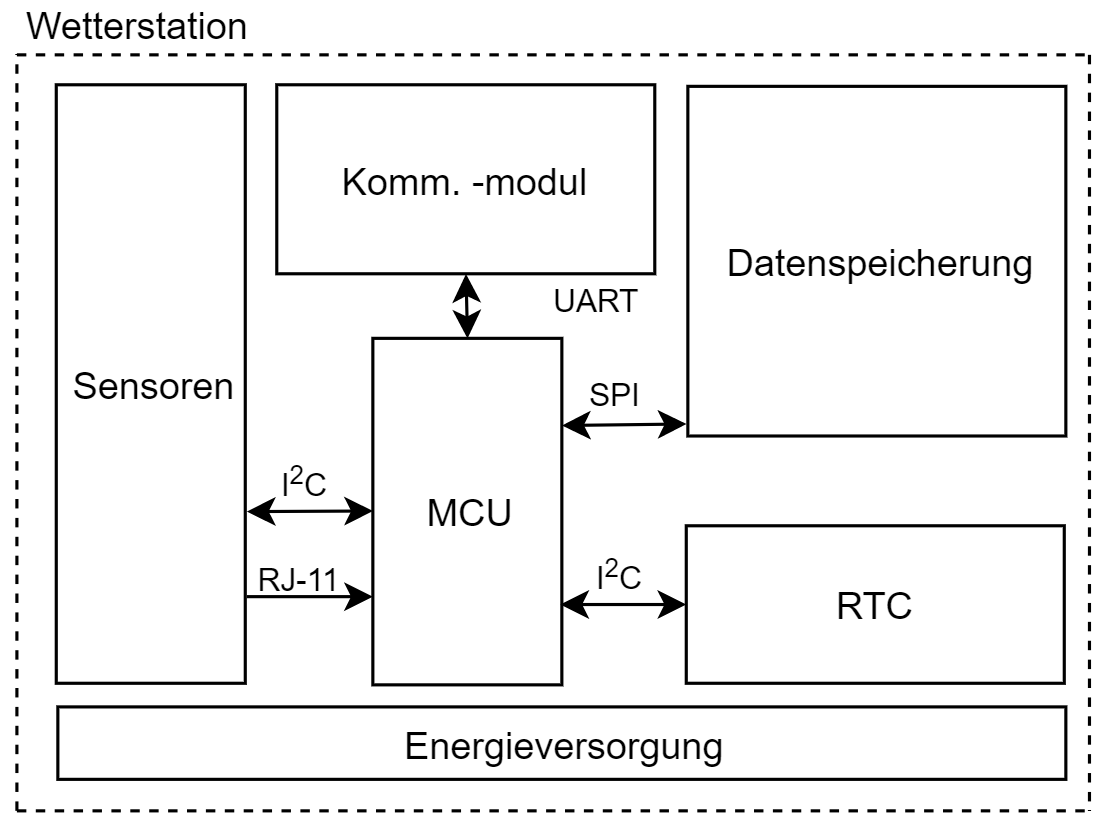
\includegraphics[width=0.9\textwidth]{graphics/Konzeptdiagramme/Grundkonzept.PNG}
\caption{Grundkonzept}
\label{fig:grundkonzept}
\end{figure}


Das gesamte Grundkonzept ist, wie in der Abbildung \ref{fig:grundkonzept} grafisch dargestellt, modular aufgebaut. Auf alle einzelnen Module wird folgend spezifischer eingegangen und genauer erklärt wie die partiellen Module funktionieren, sowie auch das gesamte System aufgebaut ist.\\

Als Zentralrecheneinheit wird eine \textit{Micro-Controller-Unit (MCU)} verwendet. Dieser ist dafür verantwortlich, dass die Daten richtig verarbeitet und an das dementsprechende Modul weitergeleitet werden. Die Messdaten werden in digitaler Form vom Modul \textit{Sensoren} über das I$^{2}$C-Interface an die \textit{MCU} übertragen. Dieser fügt mit dem \textit{Real-Time-Clock (RTC)} einen Timestamp hinzu, wobei anschließend die Daten in der \textit{Datenspeicherung} nichtflüchtig gespeichert werden. Über das \textit{Kommunikationsmodul} können dann die Daten von Nutznießern abgefragt werden.\\

Das Kommunikationsmodul beinhaltet momentan nur das USB-Interface für eine Kommunikation nach außen, wie auch zu Debbug-Zwecken des Programms. Auch die Energieversorgung wurde noch nicht implementiert und wurde folgend auch noch nicht genauer erläutert. Diese zwei Teile des Projektes werden in einem weiterführendem Projekt realisiert.\\

\newpage

\begin{figure}[hbtp]
\centering
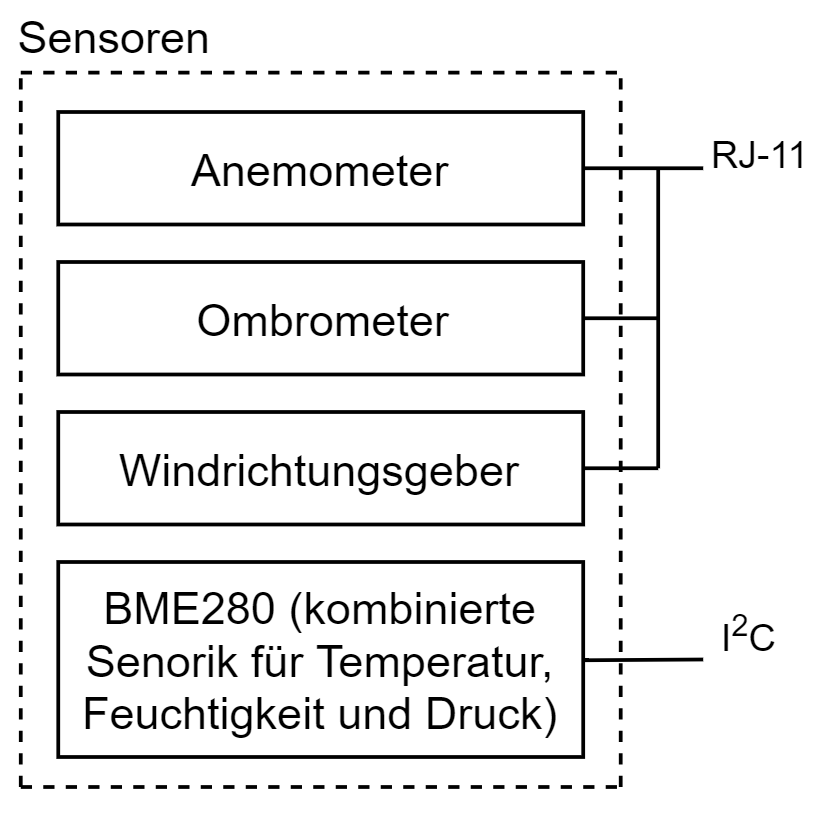
\includegraphics[width=0.6\textwidth]{graphics/Konzeptdiagramme/Sensoren.PNG}
\caption{Modul Sensoren mit den verwendeten Sensoren und Messfühlern}
\label{fig:Sensoren}
\end{figure}

Um eine bessere Übersicht über die verwendeten Sensoren zu geben, wie sie angeschlossen sind und wo sie sich in der gesamten Abstraktion des Konzeptes befinden dient Abb. \ref{fig:Sensoren}. Genauere Spezifikationen der Sensorik werden in den folgenden Kapiteln erläutert.

\newpage
\subsection{Prototyping}
\begin{figure}[hbtp]
\centering
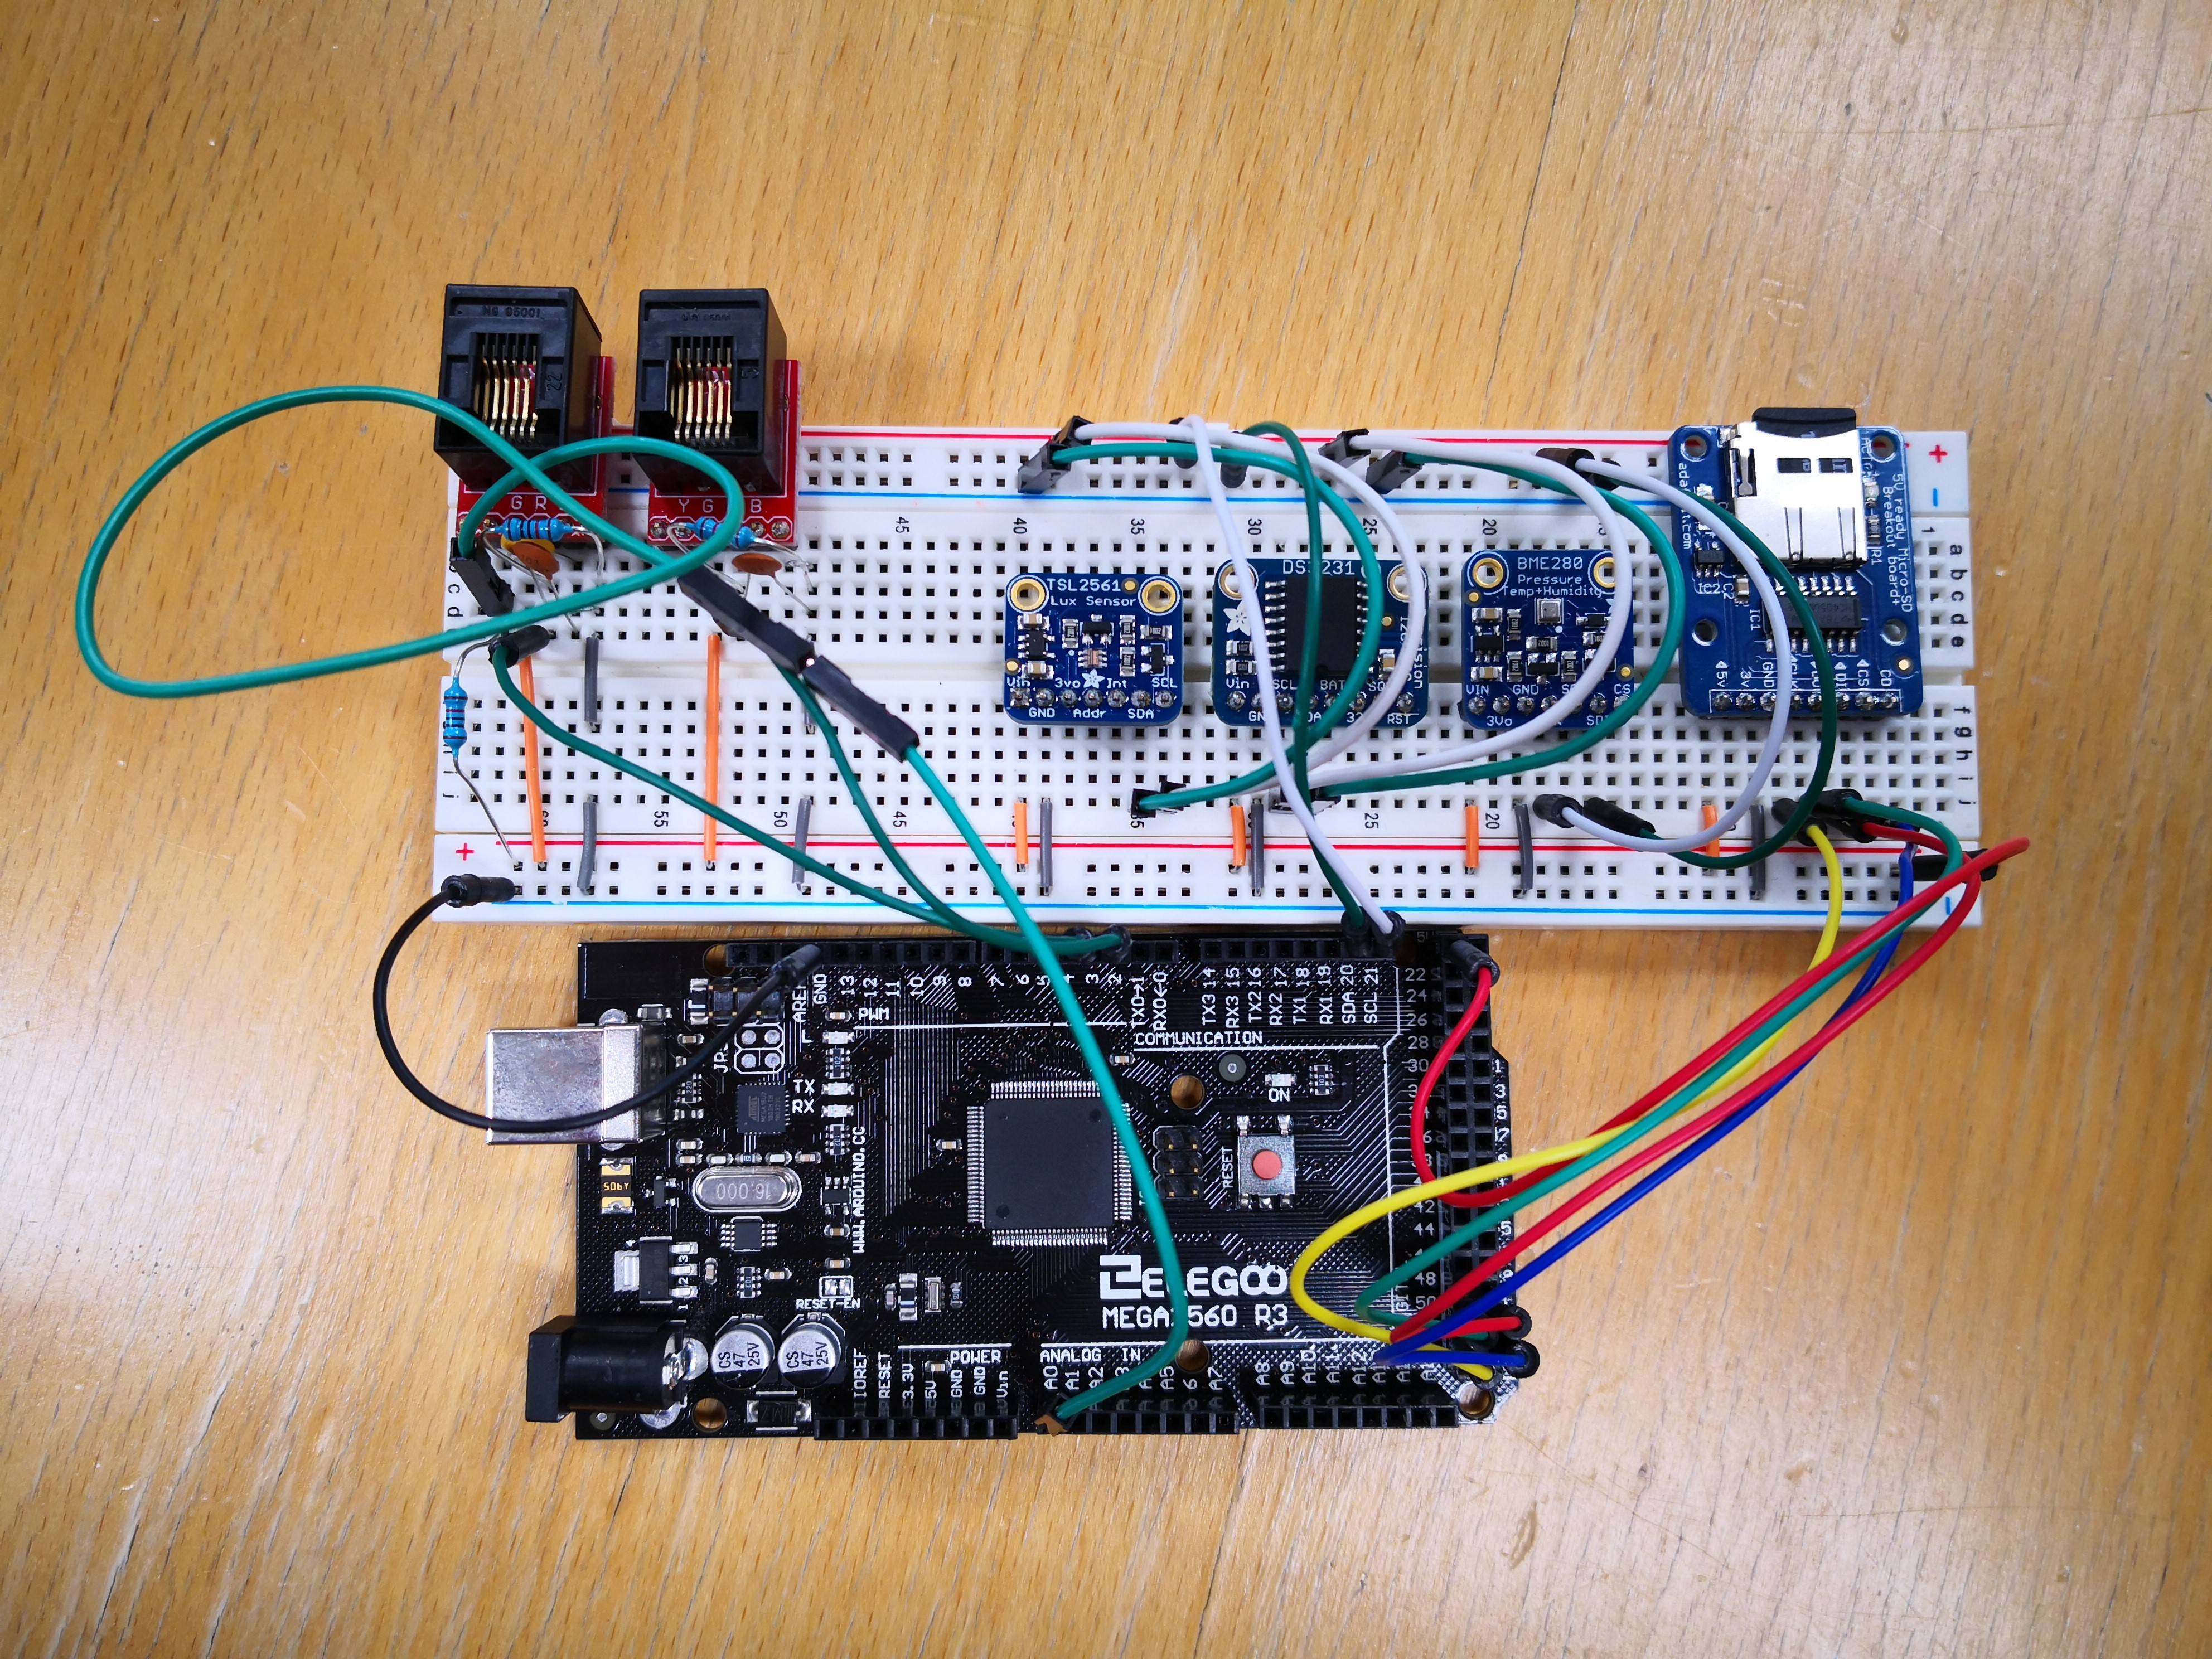
\includegraphics[width=0.9\textwidth]{graphics/prototyping/IMG_20190118_105725.jpg}
\caption{Prototyping mittels Breakoutboards}
\end{figure}

\section{Interfaces} \label{chap:interfaces}
\subsection{SPI (Serial Peripheral Interface)}
\label{subsubsec:spi}
\begin{minipage}{0.48\textwidth}
Das \textit{Serial Peripheral Interface} ist ein synchrones serielles Datenprotokoll (Datenbus) bestehend aus drei Datenleitungen zur Datenübertragung. Diese sind, wie in Abbildung \ref{fig:spi} zu sehen, \textbf{MISO} (Master In Slave Out), \textbf{MOSI} (Master Out Slave In) und \textbf{SCLK} (Serial Clock). Auf dem Breakoutboard (Abb. \ref{fig:muSDBreakout}) sind die Pins mit \textbf{DI} (Data In), \textbf{DO} (Data Out) und \textbf{CLK} (Clock) beschrieben. Zu den Datenleitungen wird noch eine \textbf{SS}- (Slave Select) oder auch \textbf{CS}-Leitung (Chip Select) benötigt. Damit wird vom Master aus den zur momentanen Kommunikation nötigen Slave selektiert. Große Vorteile von SPI sind die Vollduplexfähigkeit und das Taktfrequenzen bis in den MHz-Bereich reichen. \cite{spi}\cite{Wikipedia2018spi}\\
\end{minipage}
\begin{minipage}{0.51\textwidth}
\centering
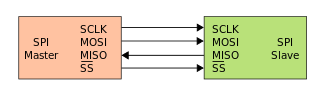
\includegraphics[width=\textwidth]{graphics/Datenspeicherung/spi_master_slave.png}
\captionof{figure}{Einfacher SPI-Datenbus \cite{Wikipedia2018spi}}
\label{fig:spi}
\end{minipage}
\todo[inline]{Möglicherweise noch die Taktfrequenz angeben, resp. die Einstellungen des SPI-Protokolls}
\subsection{I$^{2}$C}
\section{MCU}
Die Micro Controller Unit (MCU) ist der zentrale Bestandteil für die Kommunikation, resp. für den Datenaustausch zwischen den unterschiedlichen Modulen. Sie interpretiert die Signale der Sensoren und rechnet sie in die interessierenden Messwerte um. Dann weist die MCU jedem Messwert einen Zeitstempel über das RTC zu und übergibt diesen der Datenspeicherung. Wenn die Daten vom Kommunikationsmodul angefordert werden, liest die MCU die Datenspeicherung aus und übergibt sie dem Kommunikationsmodul.\\

{\begin{minipage}[b][130pt][t]{0.5\textwidth}
Für die Entwicklung der MCU wird ein Arduino Mega Board verwendet. Der Vorteil besteht darin, dass elementare Bauteile (Hardware) bereits implementiert sind, wie z.B. Oszillator, der USB-Anschluss und die PCB-Connectors für ein schnelles Prototyping. Die wichtigsten technischen Daten sind in der Tabelle \ref{tab:arduinoMega_technischeDaten} aufgelistet.\\
\end{minipage}}
\hfill
{\begin{minipage}[b][130pt][t]{0.49\textwidth}
\centering
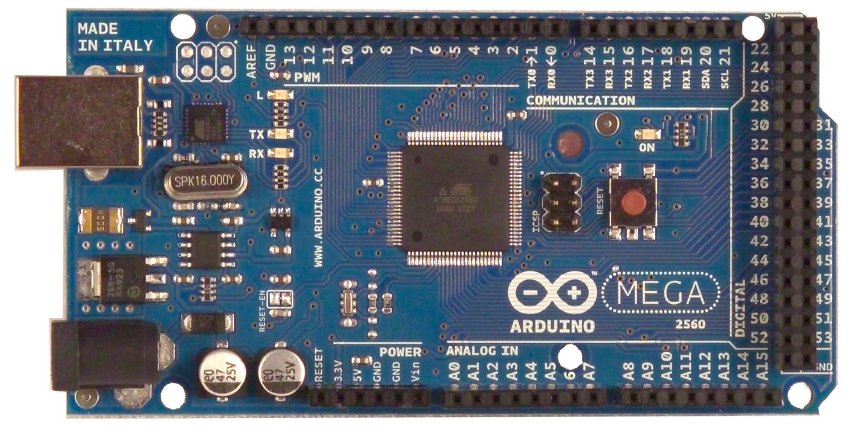
\includegraphics[width=0.99\textwidth]{graphics/MCU/arduino_mega.png}
\captionof{figure}{Arduino Mega Board \cite[S.1]{arduinoMega}}
\label{fig:arduinoMega}
\end{minipage}}

\begin{table}[h]
\centering
\caption{Technische Daten \cite[S.3]{arduinoMega}}
\begin{tabular}{|l|l|}
\hline 
Microcontroller & ATmega2560 \\ 
\hline 
Operating Voltage & 5V \\ 
\hline 
Digital I/O Pins & 54  \\ 
\hline 
Analog Input Pins & 16 \\ 
\hline 
Flash Memory & 256 KB, 8 KB werden vom bootloader benötigt\\ 
\hline 
SRAM & 8 KB \\ 
\hline 
EEPROM & 4 KB \\ 
\hline 
Clock Speed & 16 MHz \\ 
\hline 
\end{tabular}
\label{tab:arduinoMega_technischeDaten}
\end{table}

\section{RTC}
\label{chap:RTC}
Um die gewonnenen Messdaten mit einem Zeitstempel zu versehen, wird eine \textbf{RTC} (\textit{real time clock}) benötigt. Um eine möglichst kleine Abweichung zu haben, wird eine hohe Präzision vorausgesetzt. Ausserdem soll die \textbf{RTC} über das in Kapitel \ref{subsubsec:I2C} erwähnte \textbf{I$^2$C}-Bus angesteuert werden. Aus diesen Gründen wurde der \textbf{DS3231} implementiert, da dieser als Präzisions-\textbf{I$^2$C}-\textbf{RTC} die Anforderungen erfüllt. Die hohe Präzision des \textbf{DS3231} wird mit einem internen Temperatursensor erreicht, welcher Temperaturbedingte Abweichungen des Oszillators kompensiert. Zu sehen ist der \textbf{DS3231} mit seinen Anschlüssen in Abbildung \ref{fig:DS3231}.

\begin{figure}[h]
\centering
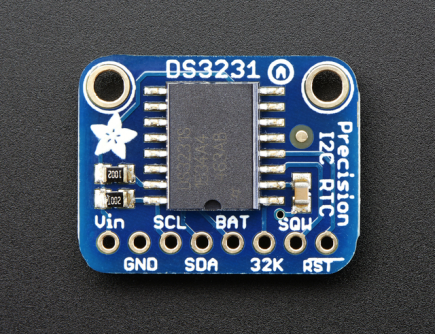
\includegraphics[width=0.4\linewidth]{graphics/DS3231.png}
\caption{\textbf{DS3231} mit seinen Anschlüssen \cite{DS3231DS}.}
\label{fig:DS3231}
\end{figure}

Die Anschlüsse des \textbf{DS3231} sind \textbf{VCC}, \textbf{GND}, \textbf{SCL}, \textbf{SDA}, \textbf{BAT}, \textbf{32K}, \textbf{SQW} und \textbf{RST}. \textbf{VCC} und \textbf{GND} werden für die Speisung benötigt. \textbf{SCL} und \textbf{SDA} sind Anschlüsse für den \textbf{I$^2$C}-Bus. \textbf{BAT} ist der positive Anschluss der Knopfbatterie, worüber deren Zustand kontrolliert werden, etwas anderes gespiesen oder eine andere Battery als Backup angeschlossen werden kann. \textbf{32K} ist ein Anschlusspin um den Output des 32kHz-Oszillators des \textbf{RTC} abzugreifen, was jedoch nicht verwendet wird. \textbf{SQW} ist ein zusätzlicher Output- oder Interrupt-Pin, welcher jedoch auch nicht verwendet wird. \textbf{RST} wird verwendet, um ein externes Element zu reseten oder als Indikator wenn die Hauptspeisung unterbrochen wird. \cite{DS3231DS}\\

\newpage
Die relevanten Spezifikationen des Chips sind in Tabelle \ref{tab:DS3231} aufgelistet.\\

\begin{table}[h]
\begin{tabular}{llllll}
\hline 
\textbf{Parameter} & \textbf{Min.} & \textbf{Typ.} & \textbf{Max.} & \textbf{Einheit} & \textbf{Condition} \\ 
\hline 
VCC & 2.3 & 3.3 & 5.5 & V &  \\ 
VBAT & 2.3 & 3 & 5.5 & V &  \\ 
Active Supply Current &  &  & 200 & $\mu$A & 3.63 V \\ 
 &  &  & 300 & $\mu$A & 5.5 V \\ 
Standby Supply Current &  & & 110 & $\mu$A & 3.63 V \\ 
 &  &  & 170 & $\mu$A & 5.5 V \\ 
Crystal Aging &  & $\pm$ 1 &  & ppm & First Year \\ 
 &  & $\pm$ 5 &  & ppm & 0-10 Years \\ 
Active Battery Current &  &  & 70 & $\mu$A & 3.63 V \\ 
 &  &  & 150 & $\mu$A & 5.5 V \\ 
Timekeeping Battery Current &  & 0.84 & 3 & $\mu$A & 3.63 V \\ 
 &  & 1 & 3.5 & $\mu$A & 5.5 V \\ 
\hline 
\end{tabular} 
\caption{Spezifikationen des \textbf{DS3231} \cite{DS3231DS}.}
\label{tab:DS3231}
\end{table}

Tabelle \ref{tab:DS3231} zeigt die für das Projekt relevanten Spezifikationen des \textbf{DS3231}. Wichtig ist, dass die Alterung des Oszillators zu einem Fehler führt, dieser jedoch im ppm-Bereich liegt und somit erst über viele Jahre hinweg bemerkbar wird.

\subsection{Implementation in die Firmware}
Für die Implementation wurde die bereits existierende Library \textbf{RTClib} von Adafruit in die Firmware integriert. Anschließend konnte das Headerfile <Adafruit\_RTClib.h> inkludiert werden und mit der Funktion \textit{TimeStamp getTimeStamp()} der aktuelle Zeitstempel abgerufen werden. \\
Beim flashen des Programms wird die RTC mit der Uhr des angeschlossenen Computers synchronisiert, weshalb es durch die Übertragungsverzögerung zu einer Abweichung kommt, welche der Dauer des flashens entspricht.
\section{Sensoren}
\label{chap:Sensoren}
\subsection{Messen der Lufttemperatur}
\subsection{Ermittlung der Niederschlagsmenge}
Dieses Unterkapitel befasst sich mit der Realisierung der Niederschlagsmessung. Diese soll nach einem Kipplöffelprinzip funktionieren und gemäss definierten Zielen eine Genauigkeit von $\pm$100 ml/$m^2$ aufweisen. Ausserdem soll als alternative zusätzlich ein Messbecher an der Wetterstation installiert werden, damit der Bauer die Niederschlagsmenge anhand einer Skala ablesen kann. In einem ersten Schritt soll das Kipplöffelprinzip näher erläutert und mit einem Selbstbau die Funktionsweise getestet werden. Anschliessend soll ein gekaufter Sensor die Wetterstation erweitern und die Implementation in der Firmware thematisiert werden. Zu guter Letzt soll die Validierung des Teilsystems folgen.
\subsubsection*{Das Kipplöffelprinzip}
Das Prinzip des Kipplöffels wird in Abbildung \ref{fig:Kipp} graphisch dargestellt.

\begin{figure}[h]
\centering
\includegraphics[width=0.8\linewidth]{graphics/Kipploeffel.png}
\caption{Darstellung des Kipplöffelprinzips}
\label{fig:Kipp}
\end{figure}

Abbildung \ref{fig:Kipp} zeigt das Kipplöffelprinzip. Der Kipplöffel (\glqq 3)\grqq) besteht im Grunde aus zwei Löffeln und ist in der Mitte drehbar mit dem Gehäuse befestigt (\glqq 4)\grqq). Regenwasser wird über eine Öffnung im Gehäusedeckel (Trichter, \glqq 1)\grqq) zum Kipplöffel befördert (\glqq 2)\grqq). Ist der Löffel mit Regenwasser gefüllt, so kippt dieser aufgrund des Gewichts und leert das Wasser über eine Öffnung im Gehäuseboden (\glqq 5)\grqq) aus. Durch die Kippung wird der andere Löffel in die Ausgangsposition bewegt und kann sich nun mit Wasser füllen. Mit der Hilfe von Reedkontakten und Magneten wird die Anzahl der Kippbewegungen gezählt. Die Niederschlagsmenge ergibt sich aus der Anzahl Kippbewegungen, multipliziert mit dem Volumen des Kipplöffels.
\newpage

\subsubsection*{Die Realisierung des Niederschlagsmengensensors}
Um die Funktionsweise des Niederschlagsmengensensors  zu testen, wird, wie im Pflichtenheft festgehalten, dieser in einem ersten Schritt selbst erstellt. Die Erstellung kann in vier Etappen unterteilt werden. Die erste Etappe ist die Erstellung des Kipplöffels. Die zweite Etappe folgt mit der Erstellung der Drehbaren Lagerung. Als dritte Etappe folgt der Trichter und die vierte und letzte Etappe widmet sich dem Gehäuse, wobei der Trichter ein Teil des Gehäuses darstellt. Das Gehäuse wird, bei verwendung der Eigenproduktion, erst im Projekt 6 mit dem Gehäuse der gesamten Wetterstation erstellt.
\paragraph{Etappe 1: Realisierung des Kipplöffels}
Wichtig für die Erstellung des Kipplöffels sind die Dimensionierung und die Materialwahl.
 
Das Material soll wetterbeständig, einfach bearbeitbar und günstig sein und eine möglichst glatte Oberfläche haben. Die möglichst glatte Oberfläche ist notwendig, damit das Wasser im Kipplöffel sich nicht an der Oberfläche festhält und somit gut abfliesst. Acrylglas erfüllt diese Bedingungen und ist in jedem Baumarkt erhältlich, weshalb es als Material gewählt wird.

Die Dimensionierung ist Abhängig von der gewählten Genauigkeit im Pflichtenheft. Damit eine Genauigkeit von $\pm$100 ml/$m^2$ erreicht werden kann, müssen beide Löffel des Kipplöffels bei genau 100 ml Fassungsvermögen kippen. Damit dies erreicht wird, kann man physikalisch die statische Gleichgewichtsbedingung aufstellen und daraus die Dimensionierung folgern. Dies ist jedoch ein sehr aufwändiger, komplizierter und zeitintensiver weg. Einfacher ist es, wenn der Kipplöffel extra zu gross dimensioniert und die Füllmenge im nachhinein justiert wird. Die Justierung erfolgt mittels einer in der Höhe verstellbaren Lagerung, sowie mit in der Höhe verstellbaren Schrauben im Gehäuseboden, welche die Neigung der Endposition des Kipplöffels beeinflusst. Ein weiterer Vorteil dieser Nachjustierung ist, dass auch eine andere Füllmenge einstellbar wäre.

\begin{figure}[h]
\centering
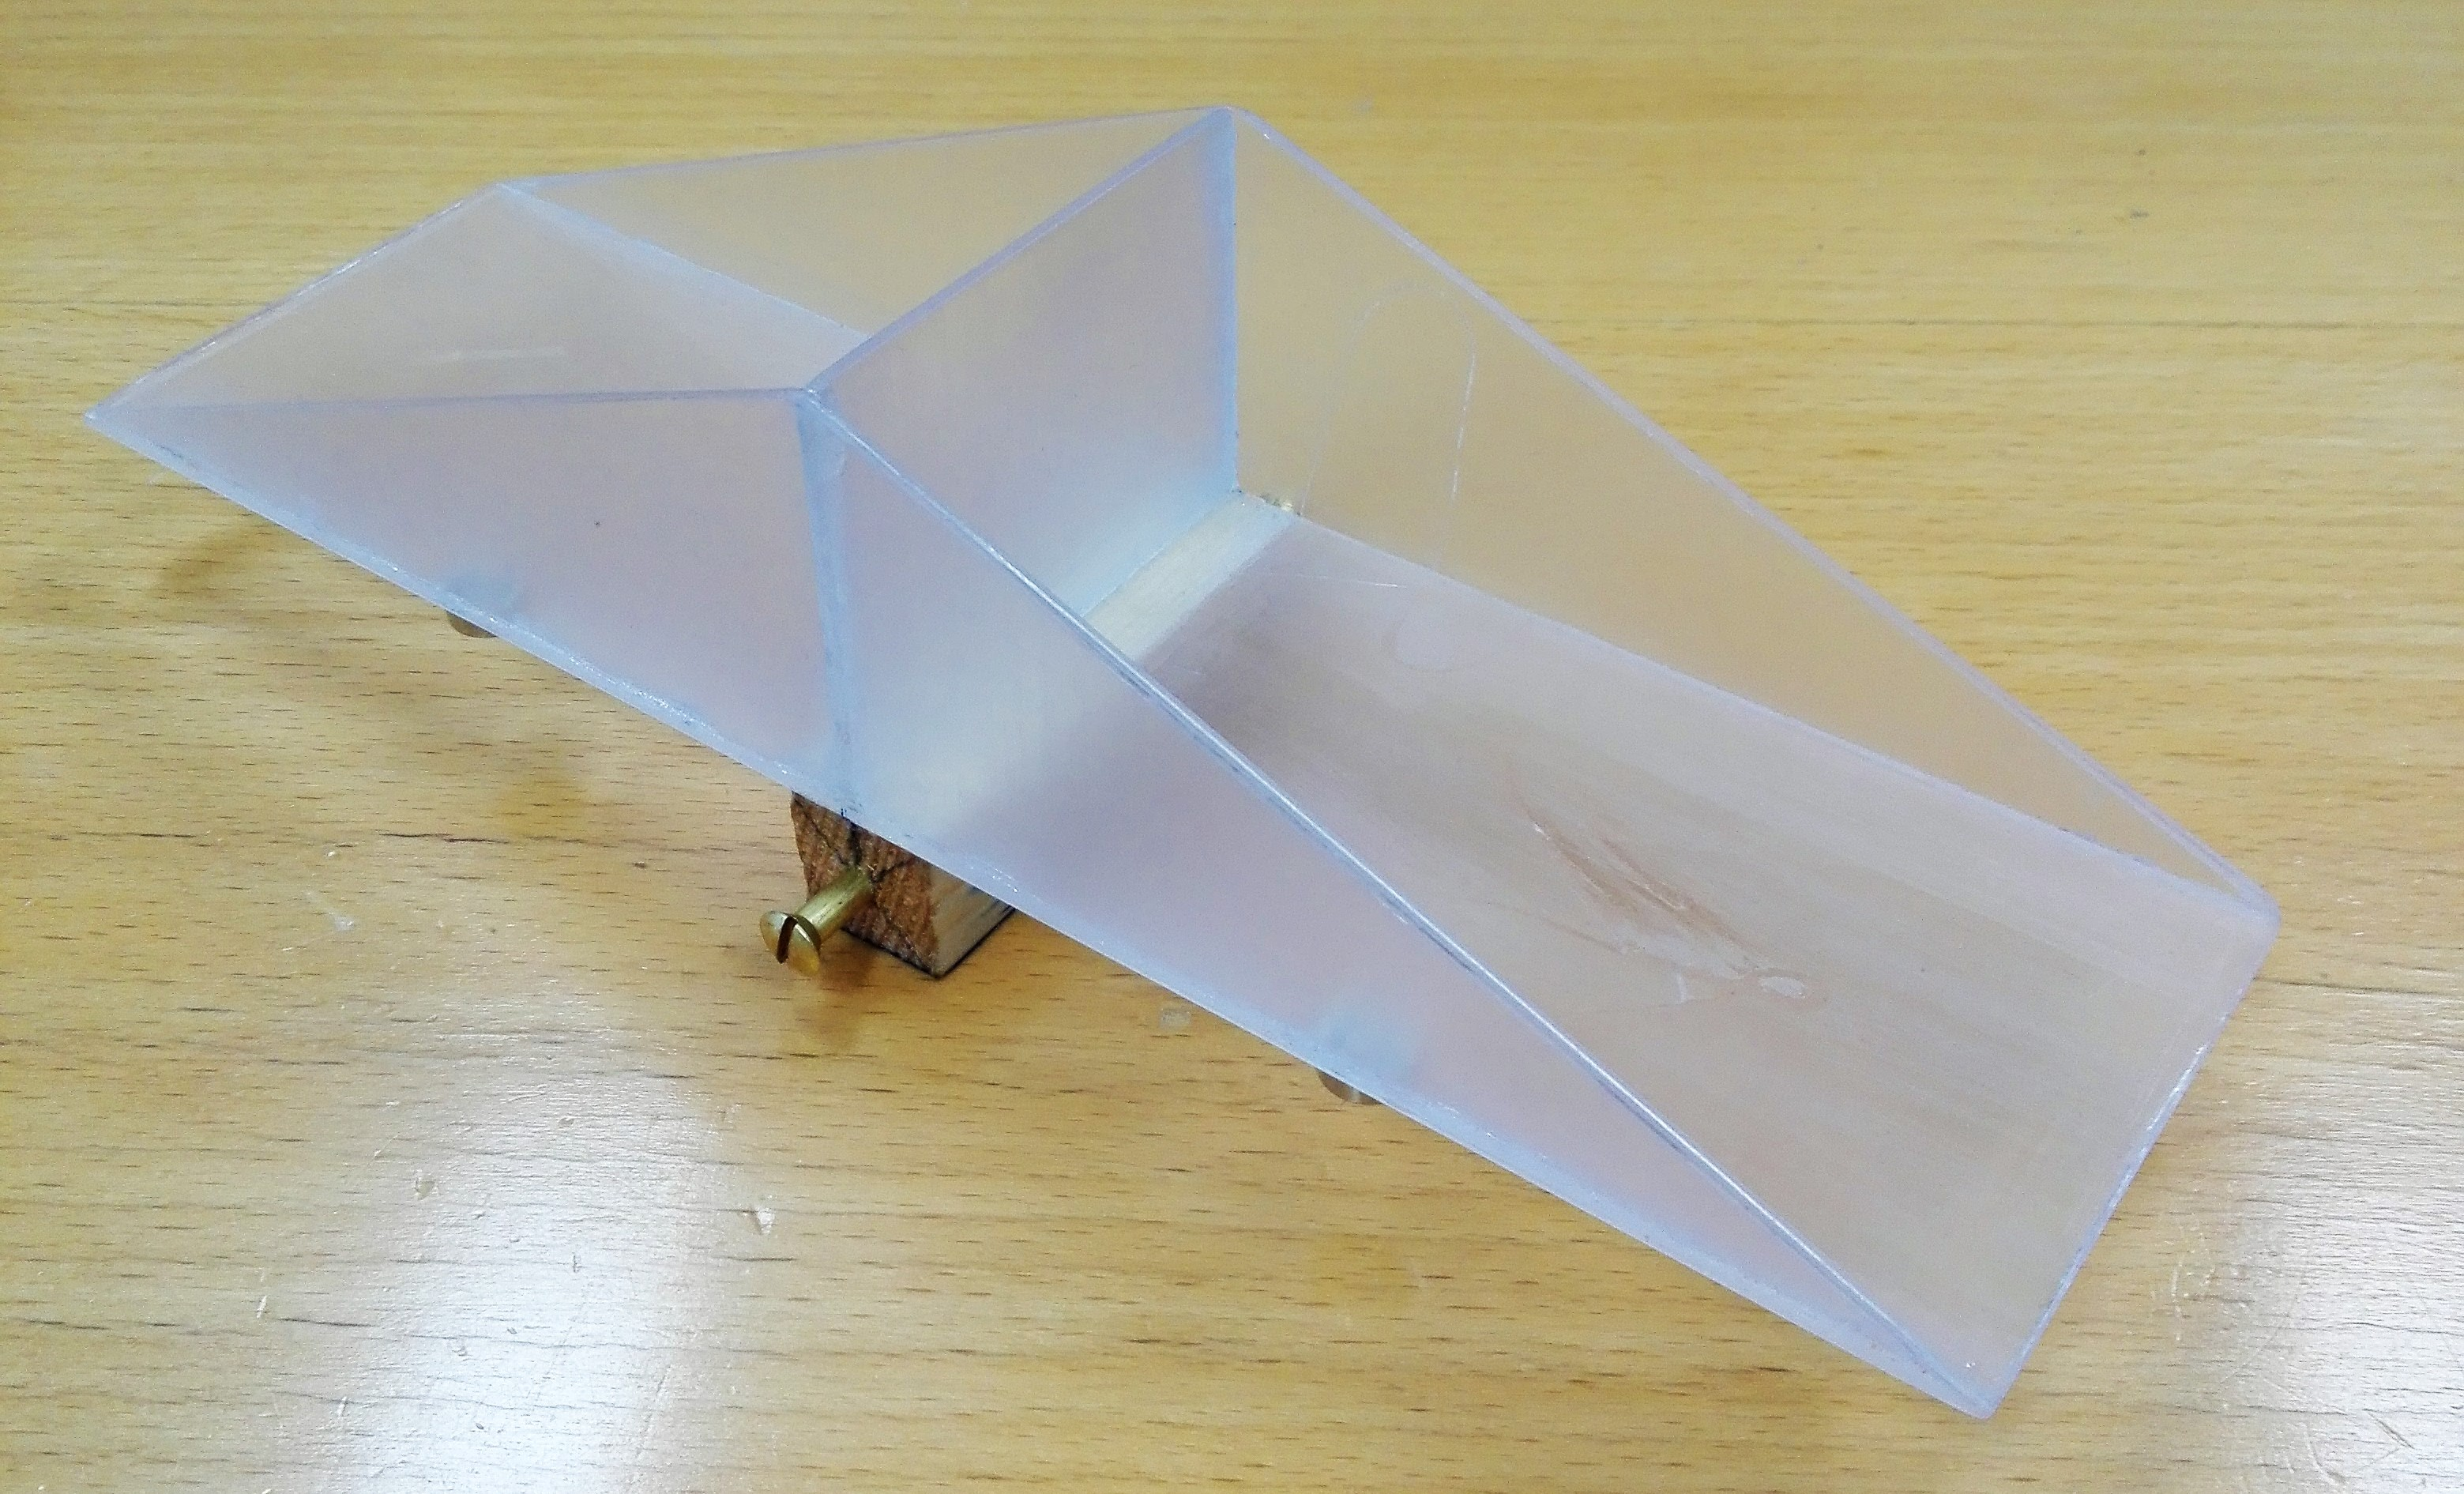
\includegraphics[width=0.8\linewidth]{graphics/Etappe1.jpg}
\caption{Selbsterstellter Kipplöffel.}
\label{fig:Etappe1}
\end{figure}

Abbildung \ref{fig:Etappe1} zeigt den selbsterstellten Kipplöffel aus Acrylglas. Die Drehachse ist mittig unter dem Kipplöffel befestigt und besteht aus einem Holzklotz mit je einer Schraube pro Seite.

\paragraph{Etappe 2: Realisierung der drehbaren Lagerung}
Die Drehbare Lagerung des Kipplöffels ist wichtig, damit der Kipplöffel auf beide Seiten kippen kann. Die Drehachse soll direkt unterhalb der Mitte des Kipplöffels befestigt sein um ein gleichmässiges Kippen zu ermöglichen. Die Höhe des Kipplöffels wird definiert durch die einstellbare Höhe der Drehachsenlagerung. 

Die Drehachse wird aus einem Stück Holz und zwei Schrauben gefertigt, wobei das Holz direkt am Kipplöffel befestigt wird. Die zwei Schrauben werden auf einem höhenverstellbarem Gerüst gelagert, so dass ein drehen möglich ist. Dieses Gerüst wird auch aus Holz gefertigt und enthält eine Metallische Fläche an der Kontaktstelle der zuvor erwähnten Schrauben, um aufkommende Reibkräfte zu verringern. Ausserdem ist dieses Gerüst höhenverstellbar über zwei mit Muttern feststellbaren Gewinden (für jede Seite eine). 

\begin{figure}[h]
\centering
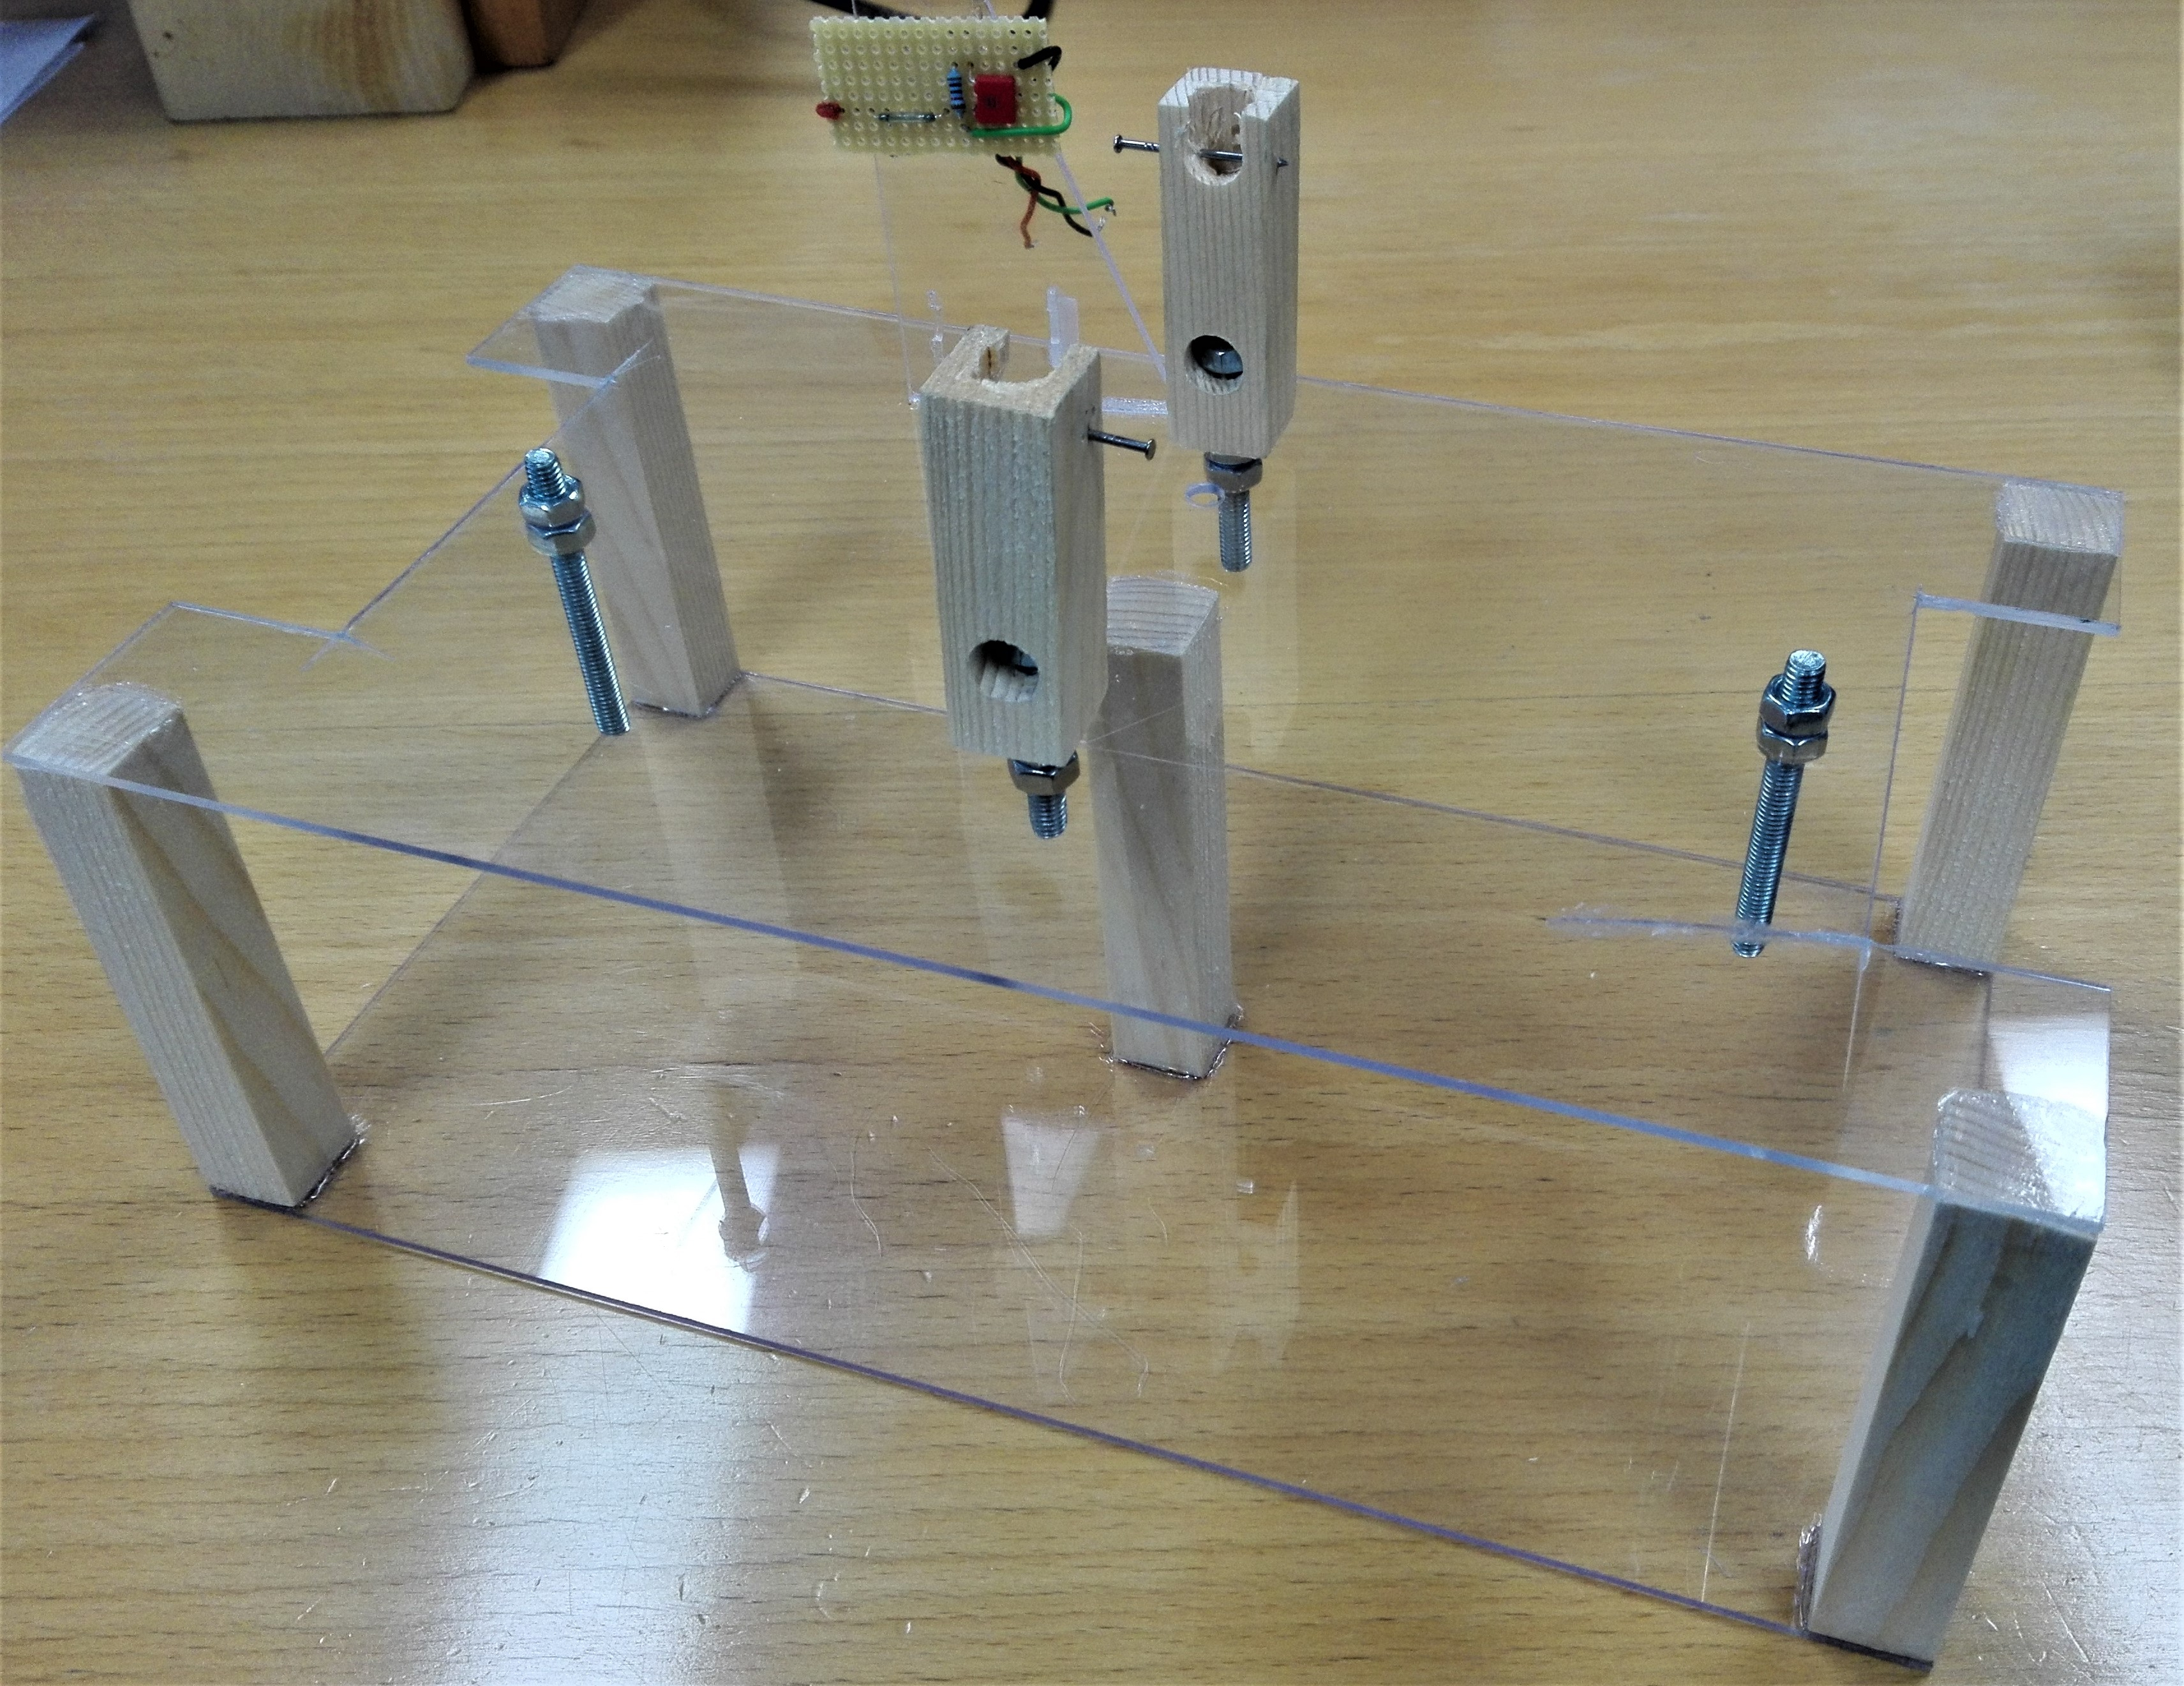
\includegraphics[width=0.8\linewidth]{graphics/Etappe2.jpg}
\caption{Selbsterstelltes Gerüst.}
\label{fig:Etappe2}
\end{figure}

Abbildung \ref{fig:Etappe2} zeigt das selbsterstellte Gerüst für die Höhenverstellbare, drehbare Lagerung des Kipplöffels. Es kann sowohl die Höhe des Kipplöffels, sowie dessen Neigung in den Endpositionen über Gewinden mit Muttern eingestellt werden. Die Schrauben des Kipplöffels kommen auf einen Stahlnagel zu liegen, womit Reibungsverluste gering gehalten werden.

\paragraph{Etappe 3: Realisierung des Trichters}
Der Trichter sorgt dafür, dass der Regen, welcher auf die Trichterfläche fällt, über der Mitte des Kipplöffels in den Löffel fliesst. Die Trichterfläche stellt gleichzeitig die Referenzfläche dar, da die gesamte Regenmenge dieser Fläche über den Kipplöffel erfasst wird. Ist diese Fläche von 1 $m^2$ abweichend, so muss in der Firmware ein Skalierungsfaktor implementiert werden, damit die Regenmenge wie gewünscht gemäss Pflichtenheft ermittelt werden kann. Der Trichter wird aus demselben Material gefertigt wie der Kipplöffel, da hier die gleichen Anforderungen gelten. Es sei angemerkt, dass der Trichter nur bei weiteren Verwendung des selbst erstellten Kipplöffels, zusammen mit dem Gehäuse der gesamten Wetterstation, erstellt wird.

\paragraph{Etappe 4: Realisierung des Gehäuses}
Das Gehäuse soll den Sensor vor ungewollten äusseren Einflüssen schützen, sowie umgebende Elektronik vor eventuellen Regenwasserspritzer. Ausserdem soll ein Schaltkreis mit Reedrelais implementiert werden, damit die Kippbewegungen von der Elektronik erfasst werden können. Es sei erwähnt, dass das Gehäuse nur bei weiteren Verwendung des selbst erstellten Sensors, zusammen mit dem Gehäuse der Wetterstation, konstruiert wird.

\paragraph{Implementierung des Schaltkreises}
Der Schaltkreis, welcher die Kippbewegungen feststellen soll, besteht im wesentlichen aus einem Reedrelais und einem Permanentmagneten. Das Reedrelais ist NO (Normally Open) und wirkt als stromkreisschliessender Schalter, sobald ein magnetisches Feld (z.B. das eines Permanentmagneten) sich in unmittelbarer Nähe befindet. Der Permanentmagnet wird auf dem Kipplöffel befestigt und das Reedrelais als Gegenstück an einem Fixpunkt in der Nähe. Wichtig dabei ist, dass das Reedrelais bei den Endpositionen des Kipplöffels nicht geschlossen ist, damit der Stromkreis geöffnet ist und Strom gespart werden kann. Das Reedrelais benötigt einen seriellen Widerstand, damit bei einem schliessen des Stromkreises kein Kurzschluss auftritt. Ausserdem soll ein Kondensator parallel zum Widerstand sein, um die Speisespannung zu glätten und so ein nutzbares Signal zu erhalten. Die Speisespannung stellt den Pegel für ein schliessen des Reedrelais, und somit auch für eine Kippbewegung dar. Um die Kippbewegungen zu zählen, kann somit entweder jede steigende oder jede fallende Flanke des Signals gezählt werden.  

\begin{figure}[h]
\centering
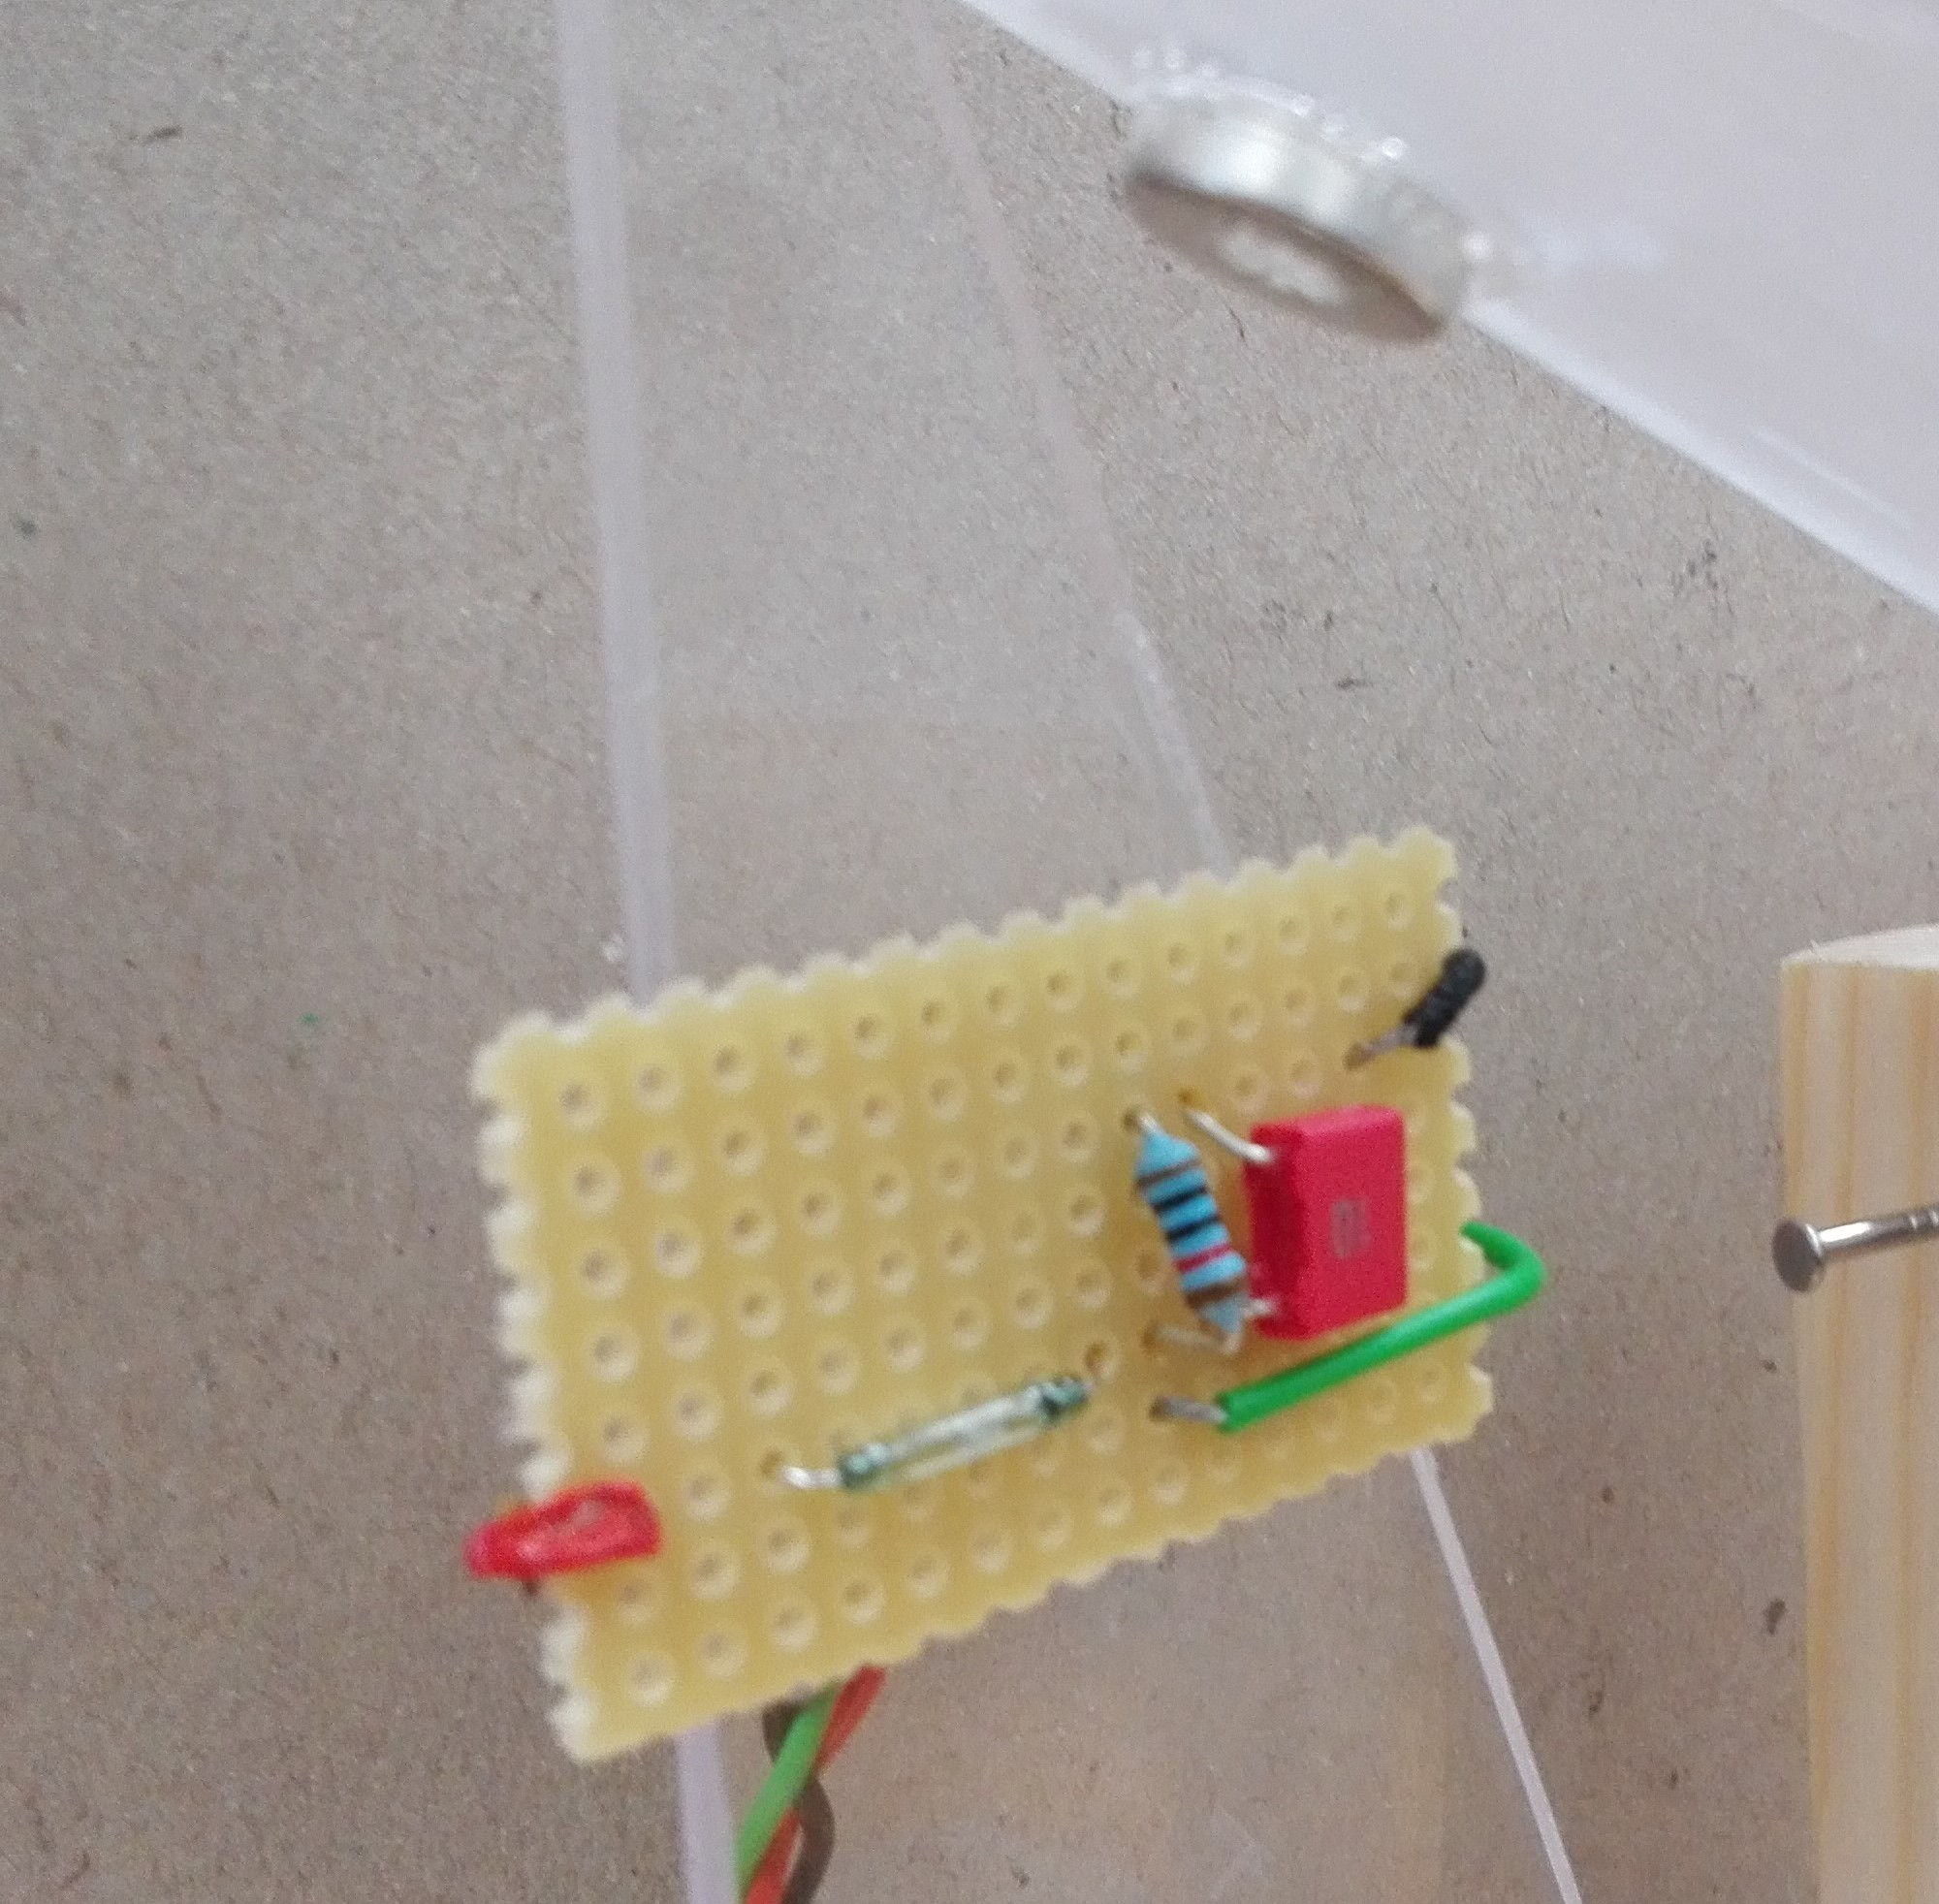
\includegraphics[width=0.4\linewidth]{graphics/KippSchalt.jpg}
\caption{Schaltkreis zur detektion der Kippbewegung.}
\label{fig:KippSchalt}
\end{figure}

Abbildung \ref{fig:KippSchalt} zeigt den Schaltkreis zur detektion der Kippbewegung. Benutzt wurde ein 10k$\Omega$ Widerstand mit einem parallel angeschlossenen 100nF Kondensator. Der Reedkontakt reagiert auf den ebenso sichtbaren Permanentmagneten, welcher an der Unterseite des Kipplöffels befestigt ist.

\paragraph{Nachteile des Selbstgebauten Niederschlagsmengensensor}
Der selbstgebaute Niederschlagssensor beweist, dass das Prinzip des Kipplöffels funktioniert. Dennoch weist der Selbstbau Mängel auf. Der verwendete Permanentmagnet muss geklebt werden, weshalb dessen Magnetfeld massiv an stärke verliert und die Schaltung deshalb äusserst nahe angebracht werden muss. Ausserdem kam es, dadurch dass keine Werkstatt zugänglich war, zu Improvisation bei nahezu allen Fertigungsschritten, was zu unkalkulierbaren Abweichungen führt. Als Beispiel sei das Spiel der drehbaren Lagerung des Kipplöffels auf dem Gerüst angeführt, was jegliche Justierungsversuche der Niederschlagsmenge beeinflusst. Aus den genannten Gründen wird vorgefertigter Sensor mit Kipplöffelprinzip verwendet.

\subsubsection*{Implentation in der Firmware}
\subsubsection*{Validierung der Niederschlagsmessung}

\newpage
\subsection{Anemometer}
{\begin{minipage}[b][650pt][t]{0.55\textwidth}
Für die Windgeschwindigkeitsmessung wurde ein Ersatz Anemometer von Froggit genommen (Abb. \ref{fig:anemometer}). Das Anschlusskabel hat einen vier poligen RJ-11 Stecker, dessen Signal über eine Buchse zum MCU geführt wird. Das Anemometer selbst hat allerdings nur zwei Anschlüsse, die Speisung (rot) und das durch einen mit einem Dauermagneten schließbaren Reedkontakt modulierte pulsförmige Ausgangssignal (grün, Abb. \ref{fig:rj11stecker}). In der Abb. \ref{fig:beschaltungAnemometer} ist ersichtlich, dass das Ausgangssignal über R1 abfällt und C1 als Spannungsstabilisierung dient. Das daraus resultierende Signal ist in der Abb. \ref{fig:rechteckpuls_anemometer} aufgezeigt. Die Windgeschwindigkeit ist nun aus der Anzahl Rechteckpulsen direkt interpretierbar:\\

Wenn über einen Zeitraum $T$ die Anzahl Pulse $A$ gemessen werden, dann kann auf die Winkelgeschwindigkeit $\omega$ nach 
\begin{equation}
\centering
\omega=\frac{A}{T}\qquad[s^{-1}]
\end{equation}
geschlossen werden. Da allerdings verschiedene Faktoren wie das Trägheitsmoment des Schalenkreuzes, Reibungsverluste bei der Drehbewegung, Verfälschung bei wechselnder Windrichtung usw. zusätzlich auf das Anemometer wirken, wird es sehr komplex die Windgeschwindigkeit exakt zu berechnen. Deshalb wird nur ein Näherungswert ermittelt und mit einem Skalierungsfaktor $SF$ korrigiert. Somit ergibt sich für die Windgeschwindigkeit $v_{Wind}$ mit Radius $r$ des Schalenkreuzes
\begin{equation}
\centering
v_{Wind} = \frac{A*r*SF}{T}\qquad[m/s].
\label{equ:berechnungWindgeschwindigkeit}
\end{equation}
Der Skalierungsfaktor $SF$ wird mittels Referenzmessungen der Windgeschwindigkeit eines digitalen Anemometers eruiert. \\
\end{minipage}}
{\begin{minipage}[b][650pt][t]{0.44\textwidth}
\centering
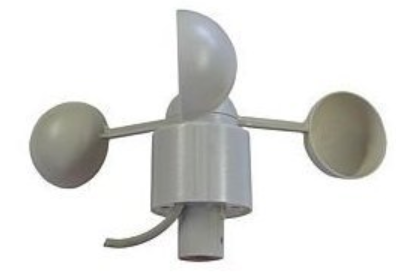
\includegraphics[width=0.9\textwidth]{graphics/Anemometer/anemometer.png}
\captionof{figure}{Anemometer \cite{AmazonAnemometer}}
\label{fig:anemometer}
\vspace{20pt}
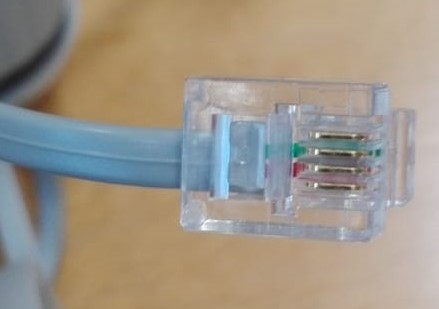
\includegraphics[width=0.9\textwidth]{graphics/Anemometer/rj_11_anschlussstecker.png}
\captionof{figure}{RJ-11 Stecker}
\label{fig:rj11stecker}
\vspace{20pt}
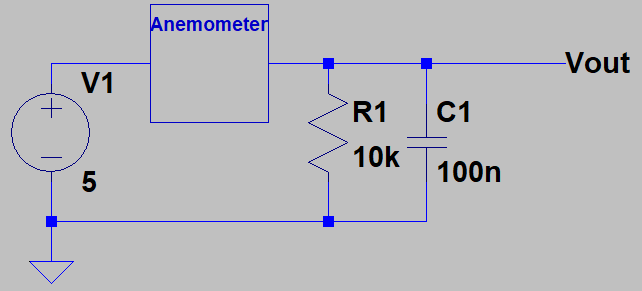
\includegraphics[width=0.9\textwidth]{graphics/Anemometer/schaltung_anemometer.png}
\captionof{figure}{Beschaltung des Ausgangs des Anemometers.}
\label{fig:beschaltungAnemometer}
\vspace{20pt}
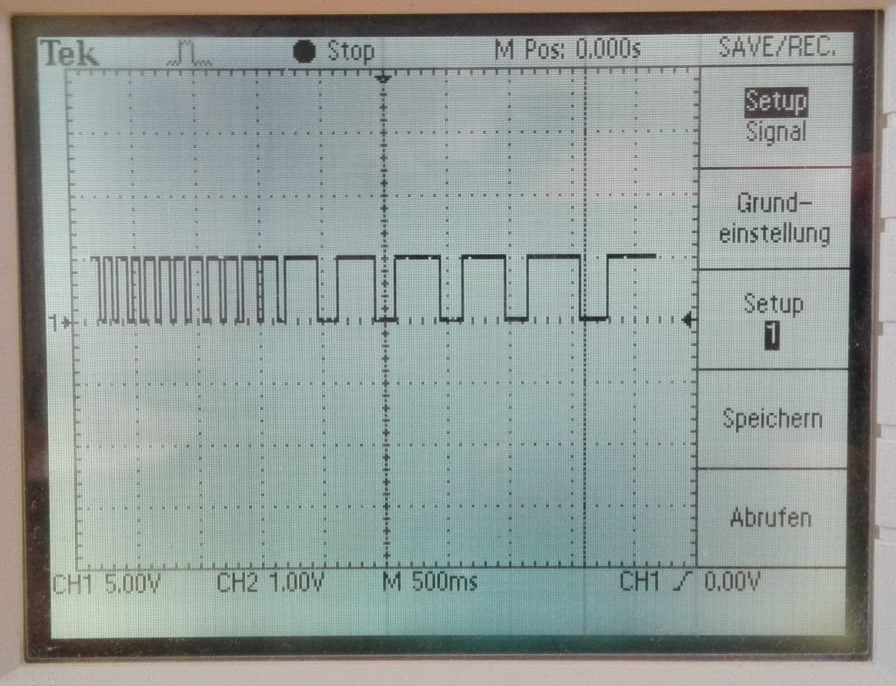
\includegraphics[width = 0.9\textwidth]{graphics/Anemometer/oszilloskop_anenometer_puls.png}
\captionof{figure}{Ausgangssignal $V_{out}$}
\label{fig:rechteckpuls_anemometer}
\end{minipage}}
\newpage

\subsubsection*{Implementation in die Firmware}
Die Implementation wurde recht simpel gehalten. Der gesamte implementierte Code für das Anemometer ist im Headerfile ''Anemometer.h'' extern deklariert und im File Anemometer.cpp initialisiert. Das Signal $V_{out}$ ist mit einen digital Pin des Atmega 2560 (Pinnummer 2 des Arduino Mega Boards) verbunden. Über einen Zeitraum von $5000ms$, auf die steigende Flanke getriggert, wird die Anzahl von Pulsen mittels Interrupt\footnote{es handelt sich hierbei um \textit{external Interrupts}.} gezählt. Dabei wird zuerst der Interrupt auf der Pinnummer 2 aktiviert, mit einem Delay von $5000ms$ gewartet, wobei bei jedem ausgelösten Interrupt die Funktion \textcolor{orange}{countWind}() ausgeführt und somit bei jeder steigenden Flanke um eins inkrementiert wird. Zum Schluss folgt die Deaktivierung des Interrupts und die Berechnung der Windgeschwindigkeit nach der Gleichung \ref{equ:berechnungWindgeschwindigkeit}.\\

\subsubsection*{Validierung}
Über eine einigermaßen konstanten Windgeschwindigkeit eines Heizlüfters/Ventilators (mit verschiedenen Stärkestufen) wurden Messpunkte des Anemometers (Abb. \ref{fig:anemometer}), sowie auch des digitalen Anemometers (Abb. \ref{fig:digitalesAnemometer}) erfasst. In der Abb. \ref{fig:messpunkteAnemometer_Vergleich} sind diese Messwerte graphisch dargestellt.\\

{\begin{minipage}[b][240pt][t]{0.65\textwidth}
\centering

\includegraphics[width=\textwidth]{graphics/placeholder.png}
\captionof{figure}{Graph der Messwerte}
\label{fig:messpunkteAnemometer_Vergleich}
\end{minipage}}
{\begin{minipage}[b][240pt][t]{0.34\textwidth}
\centering
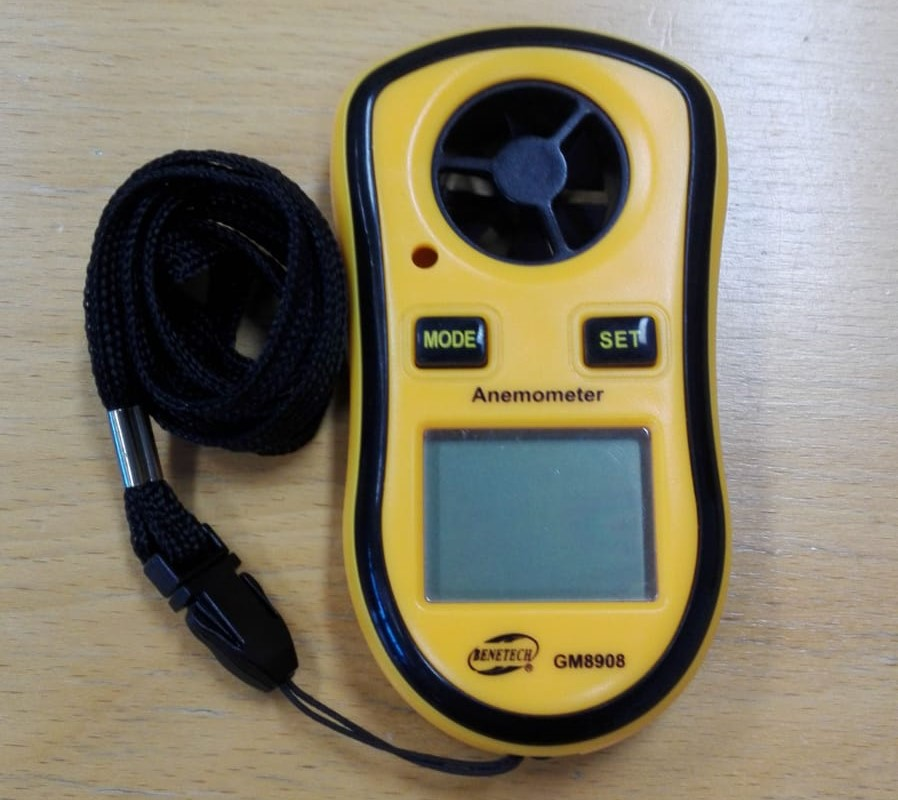
\includegraphics[width=0.9\textwidth]{graphics/Anemometer/messgeraet_anemometer.png}
\captionof{figure}{Digitales Anemometer (Benetech GM8908) mit einer Auflösung von $0.1m/s$ und einer Unsicherheit von $\pm5\%$ \cite{digitalesAnemometerBenetech}}
\label{fig:digitalesAnemometer}
\end{minipage}}
\todo[inline]{Hier muss noch die Interpretation der gemessenen Werte geschrieben werden.}
\subsection{Zählung der Sonnenstunden}

\section{Datenspeicherung}
\label{chap:data}
Die Datenspeicherung beinhaltet die gespeicherten Messwerte der Sensoren. Dafür wird als Speichermedium eine $\mu$SD-Karte verwendet, welche direkt in das 254 $\mu$SD-Breakoutboard von Adafruit gesteckt wird. Die Daten werden dann in einem *.txt-File nicht flüchtig gespeichert. Bei Beschädigung der Hardware können dann die zuletzt erfassten Daten immer noch mittels eines SD-Karten-Adapters von einem Computer ausgelesen werden. Als Kommunikationsprotokoll für das Schreiben und Auslesen der Karte wird SPI verwendet.\\
\subsection{Breakoutboard}
Das Breakoutboard (siehe Abb. \ref{fig:muSDBreakout}) kann wegen des intern implementierten \textit{CD74HC4050 high-speed logic level translators}\footnote{konvertiert eine high-level logik in eine low-level logik} mit 5V betrieben werden. Das Arduino Mega Board und das Breakoutboard werden über SPI (siehe Kapitel \ref{subsubsec:spi}) nach dem Master-Slave Kommunikationsprinzip miteinander verbunden. 
\begin{figure}[h]
\centering
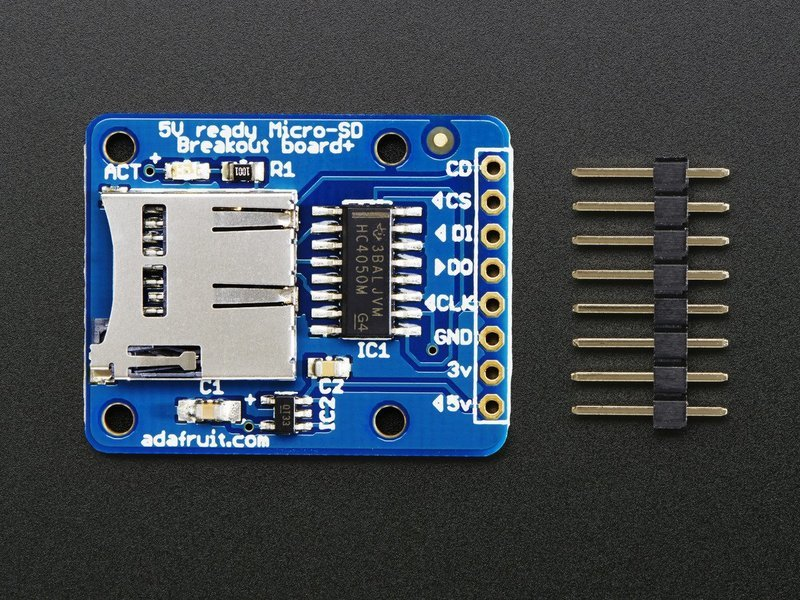
\includegraphics[width=0.5\linewidth]{graphics/Datenspeicherung/micro_sd_card_breakout.png}
\caption{254 $\mu$SD-Breakoutboard von Adafruit \cite{ladyada2018}}
\label{fig:muSDBreakout}
\end{figure}

\subsubsection{Verdrahtung}
SD-Karten erfordern viel Datenübertragung. Deshalb kann die beste Leistung erbracht werden, wenn sie an die Hardware-SPI-Pins eines Mikrocontrollers angeschlossen werden. Dabei wird es wie folgt miteinander verbunden: \cite{ladyada2018}
\todo[inline]{Hier vielleicht noch das Schema hinzufügen wie es Hardwaremässig implementiert wird.}
\begin{itemize}
\item \textbf{5V} und \textbf{GND} Pins jeweils auf die \textbf{5V} und \textbf{GND} Pins des Arduino Mega Boards
\item \textbf{CLK} auf die Pinnummer \textbf{52}
\item \textbf{DO} auf die Pinnummer \textbf{50}
\item \textbf{DI} auf die Pinnummer \textbf{51}
\item \textbf{CS} auf die Pinnummer \textbf{53}
\end{itemize}
\newpage

\subsubsection{SPI (Serial Peripheral Interface)}
\label{subsubsec:spi}
\begin{minipage}{0.48\textwidth}
Das \textit{Serial Peripheral Interface} ist ein synchrones serielles Datenprotokoll (Datenbus) bestehend aus drei Datenleitungen zur Datenübertragung. Diese sind, wie in Abbildung \ref{fig:spi} zu sehen, \textbf{MISO} (Master In Slave Out), \textbf{MOSI} (Master Out Slave In) und \textbf{SCLK} (Serial Clock). Auf dem Breakoutboard (Abb. \ref{fig:muSDBreakout}) sind die Pins mit \textbf{DI} (Data In), \textbf{DO} (Data Out) und \textbf{CLK} (Clock) beschrieben. Zu den Datenleitungen wird noch eine \textbf{SS}- (Slave Select) oder auch \textbf{CS}-Leitung (Chip Select) benötigt. Damit wird vom Master aus den zur momentanen Kommunikation nötigen Slave selektiert. Große Vorteile von SPI sind die Vollduplexfähigkeit und das Taktfrequenzen bis in den MHz-Bereich reichen. \cite{spi}\cite{Wikipedia2018spi}\\
\end{minipage}
\begin{minipage}{0.51\textwidth}
\centering
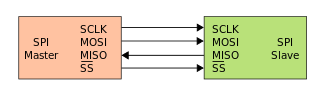
\includegraphics[width=\textwidth]{graphics/Datenspeicherung/spi_master_slave.png}
\captionof{figure}{Einfacher SPI-Datenbus \cite{Wikipedia2018spi}}
\label{fig:spi}
\end{minipage}
\todo[inline]{Möglicherweise noch die Taktfrequenz angeben, resp. die Einstellungen des SPI-Protokolls}

\subsection{$\mu$SD-Karte}
\begin{minipage}{0.44\textwidth}
\centering
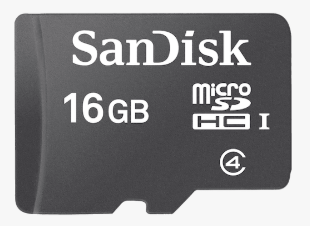
\includegraphics[width=0.4\textwidth]{graphics/Datenspeicherung/micro_sd_card_16GB.png}
\captionof{figure}{16 GB $\mu$SD-Karte \cite{musdkarte}}
\label{fig:muSDKarte}
\end{minipage}
\begin{minipage}{0.55\textwidth}
Bei der $\mu$SD-Karte muss auf die Kompatibilität mit dem Breakoutboard geachtet werden. Dafür sind folgende Kriterien zu beachten:\\
\begin{itemize}
\item Die $\mu$SD-Karte muss FAT16 oder FAT 32 formatiert sein.
\item Es sind nur die SD und SD High Capacity (SDHC) kompatibel.\\
\end{itemize}
\end{minipage}
Für die Umsetzung dieses Projektes wurde eine $\mu$SD-Karte der SD-Familie SDHC \Romannum{1} verwendet (siehe Abb. \ref{fig:muSDKarte}). SDHC sind Kapazitäten bis zu 32GB möglich und FAT32 formatiert. \cite{muSDspez} \todo[inline]{Es könnte noch auf die Anschlüsse der $\mu$SD-Karte eingegangen werden. Gäbe aber nur Sinn wenn ein Print erstellt werden muss wo das Breakoutboar nachkonstruiert wird.}
\newpage

\subsection{Implementation in die Firmware}
Für die Implementation in die Firmware, um mit dem Breakoutboard über SPI zu kommunizieren und die $\mu$SD-Karte zu beschreiben, resp. zu lesen, wurden direkt die bereits existierenden Librarys <SPI.h>\footnote{ <*.h> bezieht sich auf ein include-Verzeichnis unter dem Compiler-Installationsverzeichnis} und <SD.h> von Arduino inkludiert. In der Arduino IDE können bereits vorgefertigte Expample-Codes (siehe Abb. \ref{fig:exampleCodes}) zur weiteren Interpretation, wie mit diesen Librarys $\mu$SD-Karten gelesen und geschrieben werden können, verwendet werden.\\
\begin{figure}[h]
\centering
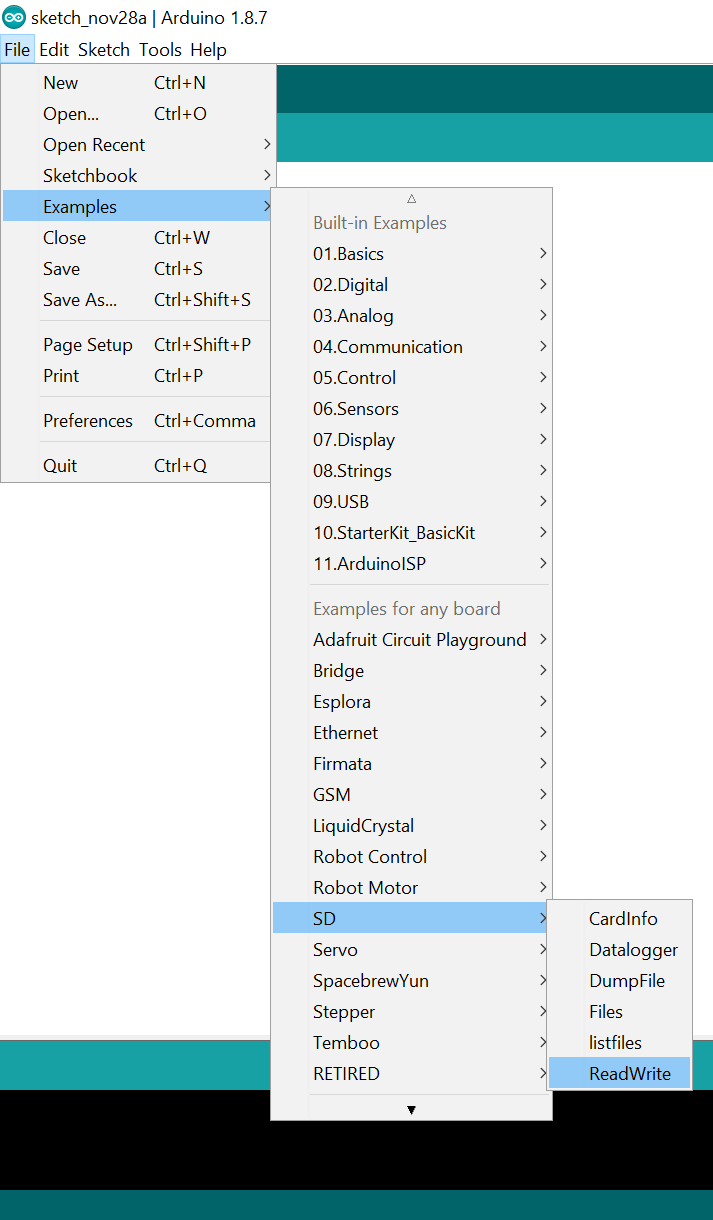
\includegraphics[width=0.48\textwidth]{graphics/Datenspeicherung/read_write_examples.PNG}
\caption{Example-Codes der Arduino IDE zum Lesen und Schreiben von SD-Karten.}
\label{fig:exampleCodes}
\end{figure}

Für eine übersichtlichere Programmstruktur und einfachere Handhabung wurden die Exampel-Codes für die korrekte Implementation angepasst und in Funktionen verpackt. Die Funktionen sind extern im Headerfile ''SDCard.h''\footnote{ ''*.h'' bezieht sich relativ auf das aktive Projektverzeichnis} deklariert und im SDCard.cpp initialisiert.
\begin{itemize}
\item \textcolor{blue}{void} \textcolor{orange}{getCardInformations}():
\item \textcolor{blue}{void} \textcolor{orange}{readFileSDCard}(\textcolor{Dandelion}{String} filename): 
\item \textcolor{blue}{void} \textcolor{orange}{writeFileSDCard}(\textcolor{blue}{double} value2save, \textcolor{Dandelion}{String} filename): 
\item \textcolor{blue}{void} \textcolor{orange}{deleteFileSDCard}(\textcolor{Dandelion}{String} filename): 
\end{itemize}
\todo[inline]{Funktionen könnten noch beschrieben werden. Noch Abklären, ob die Fußzeilen nötig sind!}
\section{Firmware}

\subsection{Development Environment}
\label{subsec:dev_envir}
Die Firmware der Wetterstation wurde im AtmelStudio 7 (Version: 7.0.1645 @2015) der Atmel Corp. und der Arduino IDE 1.8.5 geschrieben. Beide sind als Freeware erhältlich. Die Arduino IDE 1.8.5 wurde hauptsächlich verwendet, um notwendige Librarys über den \textit{Library Manager} hinzuzufügen. Dies war besonders für die Sensoren wie der BME280 notwendig. Anschliessend konnte das gesamte Projekt ins AtmelStudio importiert werden. Der Vorteil liegt darin, dass nach dem ersten PCB-Entwurf dann mittels einem ISP\footnote{In System Programmer} der Microcontroller programmierbar bleibt. Dies ist mit der Arduino IDE 1.8.5 nicht möglich.\\

%hier könnte noch die Liste der verwendeten Librarys aufgelistet werden. Falls dies überhaupt notwendig ist.

In der C++ Syntax wurde das ganze Programm objektorientiert geschrieben und aufgebaut. Grund dafür ist die Skalierbarkeit des gesamten Projekts. Das objektorientierte Design ist besser strukturiert und kann einfach und übersichtlich erweitert werden.\\


\subsection{UML-Diagramm}

\begin{figure}[hbtp]
\centering
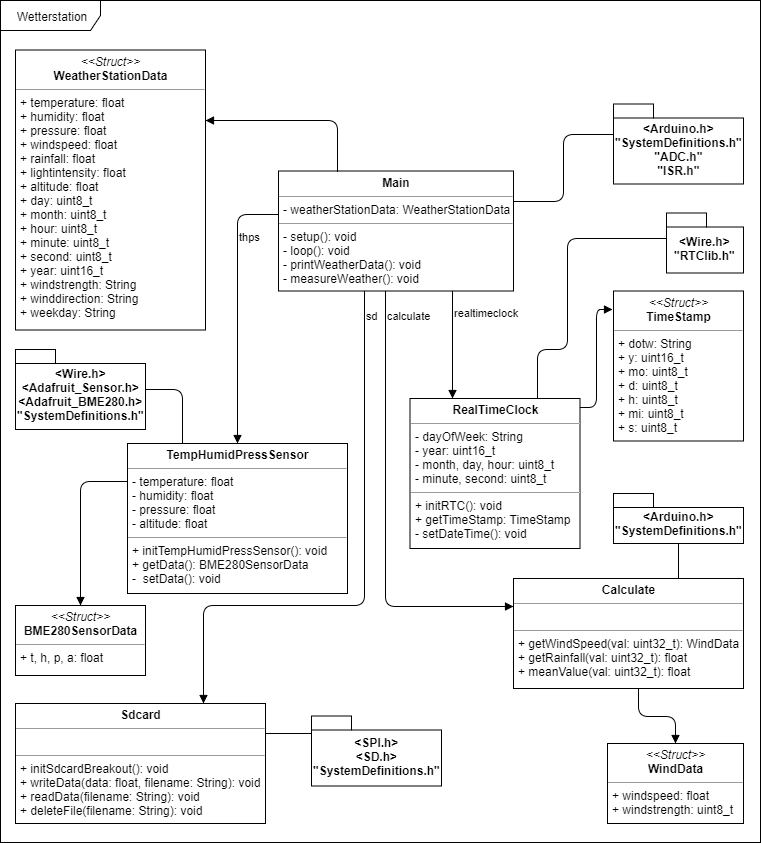
\includegraphics[width=\textwidth]{graphics/UML/UML_Diagramm_picture.PNG}
\caption{UML-Diagramm der Wetterstation}
\label{fig:uml_diagramm}
\end{figure}

Das in der Abbildung \ref{fig:uml_diagramm} dargestellte UML-Diagramm soll den Aufbau und die logischen Zusammenhänge der Firmware visualisieren. Darin wird gezeigt, welche Headerfiles bei den Klassen benötigt werden. Zudem sind die Attribute, wie auch die Funktionen mit ihren Access Specifier, Argumenten und Rückgabewerten aufgelistet. \\

Durch diese Struktur ist es möglich, adaptiv mehrere Komponenten hinzuzufügen und anzupassen. Zudem könnten somit auch mehrere Sensoren vom gleichen Typ ohne grossen weiteren Aufwand implementiert werden.\\

In der Klasse \textbf{TempHumidPressSensor} werden die Temperatur, Lufdruck und relative Luftfeuchtigkeit vom BME280 gelesen und in das Struct BME280SensorData geschrieben. Diese können dann vom \textbf{Main} über die Funktion \textit{getData()} aufgerufen werden. Über die Klasse \textbf{RealTimeClock} können die Zeitdaten vom DS3231 und zu den Messwerten zugerordnet werden. Mittels einer Klasse \textbf{Calculate} sollen notwendige Berechnungen vom restlichen Programm getrennt werden. Wenn das Programm startet, wird zuerst das \textit{setup()} aufgerufen und danach befindet sich das Programm in der Endlosschlaufe \textit{loop()}. Dieser Stil ist typisch für die Arduino IDE, wie im Kapitel \ref{subsec:dev_envir} bereits erwähnt worden ist, wird in diesem Projekt in zwei Development Environments gearbeitet.
%\section{Kommunikationsmodul}

%\section{Energieversorgung}

\section{Konzeptvalidierung}
\label{chap:valid}

\listoffigures
\listoftables
\newpage
%%---BIBLIOGRAPHY------------------------------------------------------------------------
{\sloppypar
\printbibliography[heading=bibintoc]
\label{sec:lit}
%\selectlanguage{english}				%ngerman or english
%\printbibliography[heading=bibintoc]
}

%%---APPENDIX----------------------------------------------------------------------------
\begin{appendix}
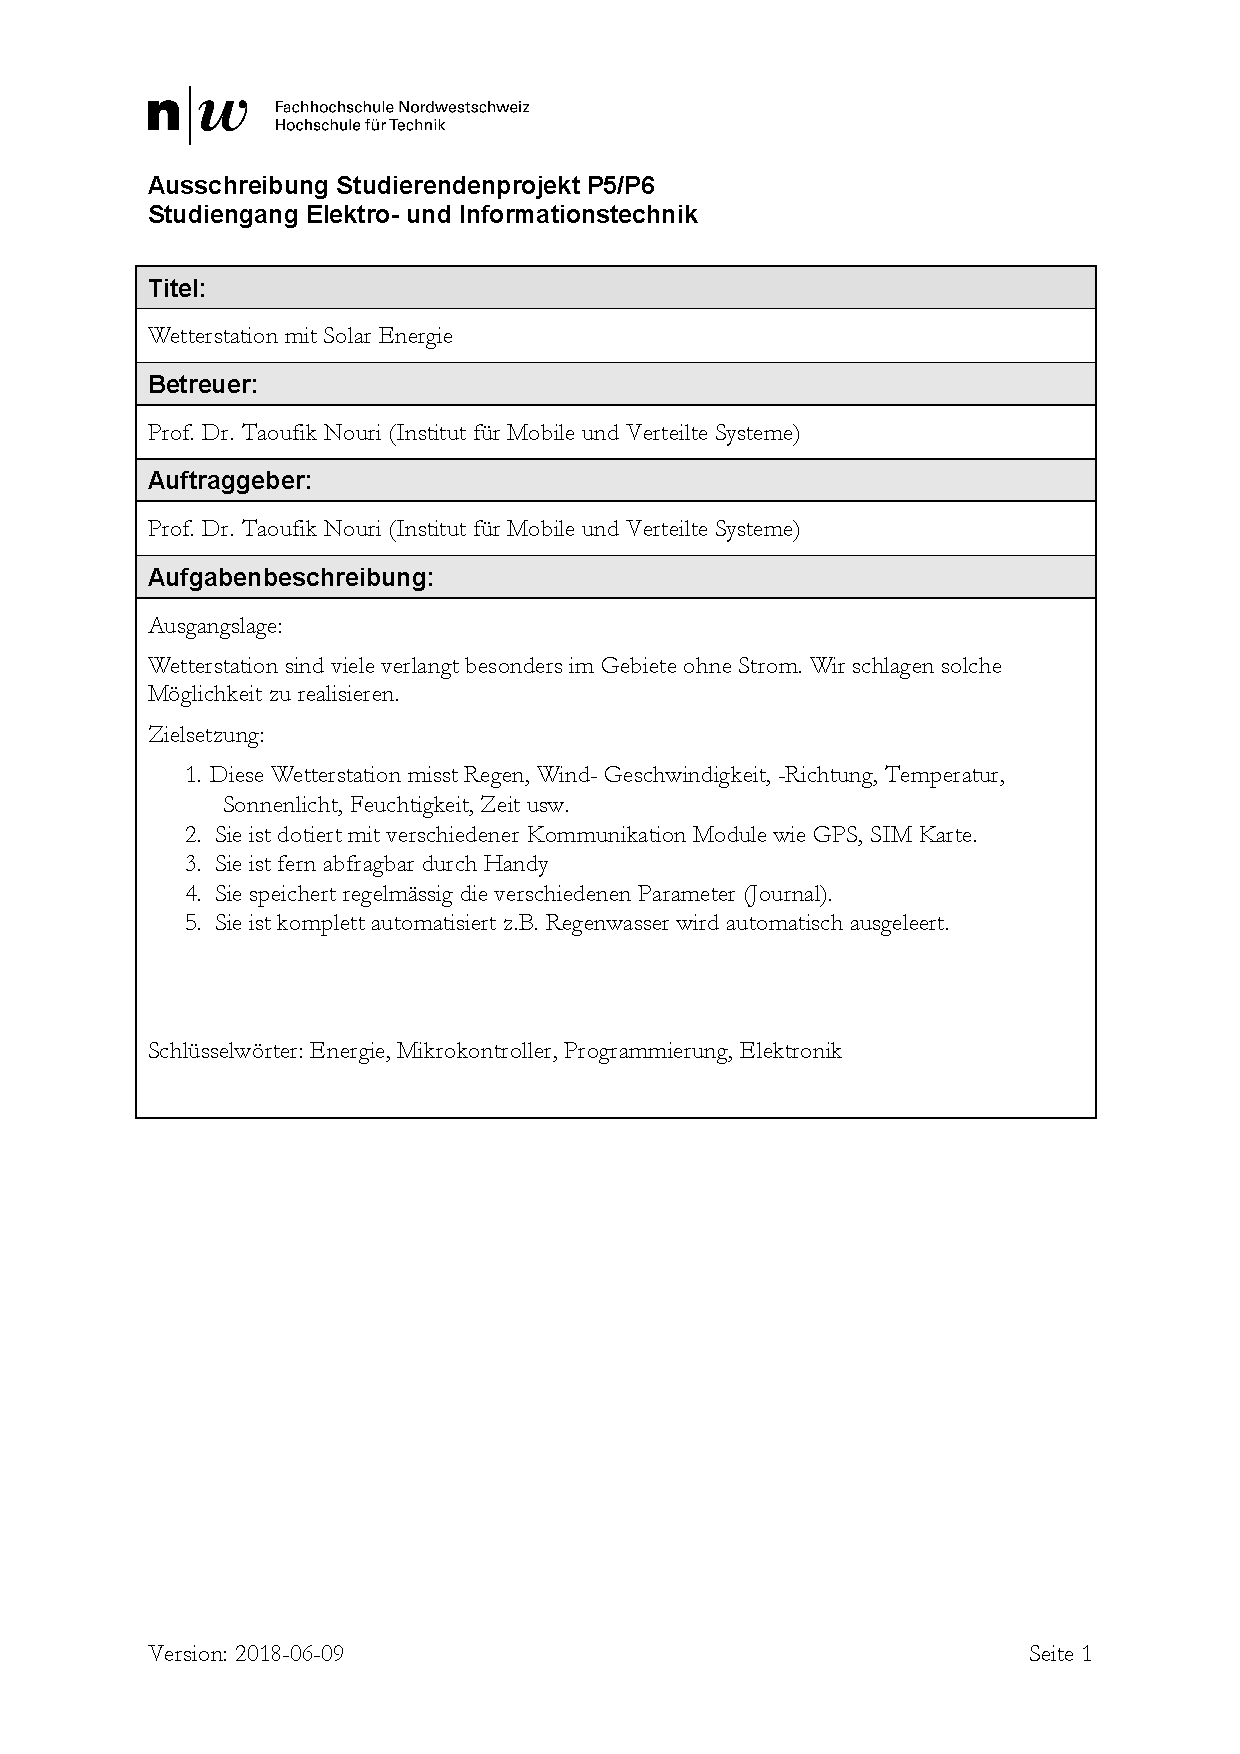
\includepdf[pages={1},nup=1x1,landscape=false,scale=0.85,offset=0 -40,pagecommand={\section{Lastenheft}\label{tab:zeitplan}\thispagestyle{myheadings}}]{appendix/Auftragsbeschreibung.pdf} 
\newpage

\end{appendix}

%%---NOTES for DEBUG---------------------------------------------------------------------
\ifdraft{%Do this only if mode=draft
%%requires \usepackage{todonotes})
\newpage
\listoftodos[\section{Todo-Notes}]
\clearpage
}
{%Do this only if mode=final
}
\end{document}
